\documentclass[12pt]{article}
\usepackage[utf8]{inputenc}
\usepackage{hyperref}
\usepackage{graphicx}
\graphicspath{ {img/} }
\usepackage[justification = centering]{caption}
\usepackage{float}
\usepackage{amsmath}
%\usepackage[version=4]{mhchem}
\usepackage{booktabs} % nice rules (thick lines) for tables
\usepackage{microtype} % improves typography for PDF
\usepackage{float}
\usepackage{multicol}

\newcommand{\labname}{458 Group 8 Nuclear Shipping\xspace}%

%\course{NPRE 448}
\title{FISHP$_3$: Fast Inherently-Safe Hybrid Propulsion and Power Plant}
\author{Louis Kissinger, Brad Ellis, and Adam Pichman \\Course: NPRE 458; Advisor: Magdi Ragheb} 
\date{February 22, 2019}
\makeatletter
\setlength{\@fptop}{0pt}
\makeatother

\begin{document}

%TITLE PAGE
\maketitle
\begin{figure}[H]                                  
    \centering                                     
    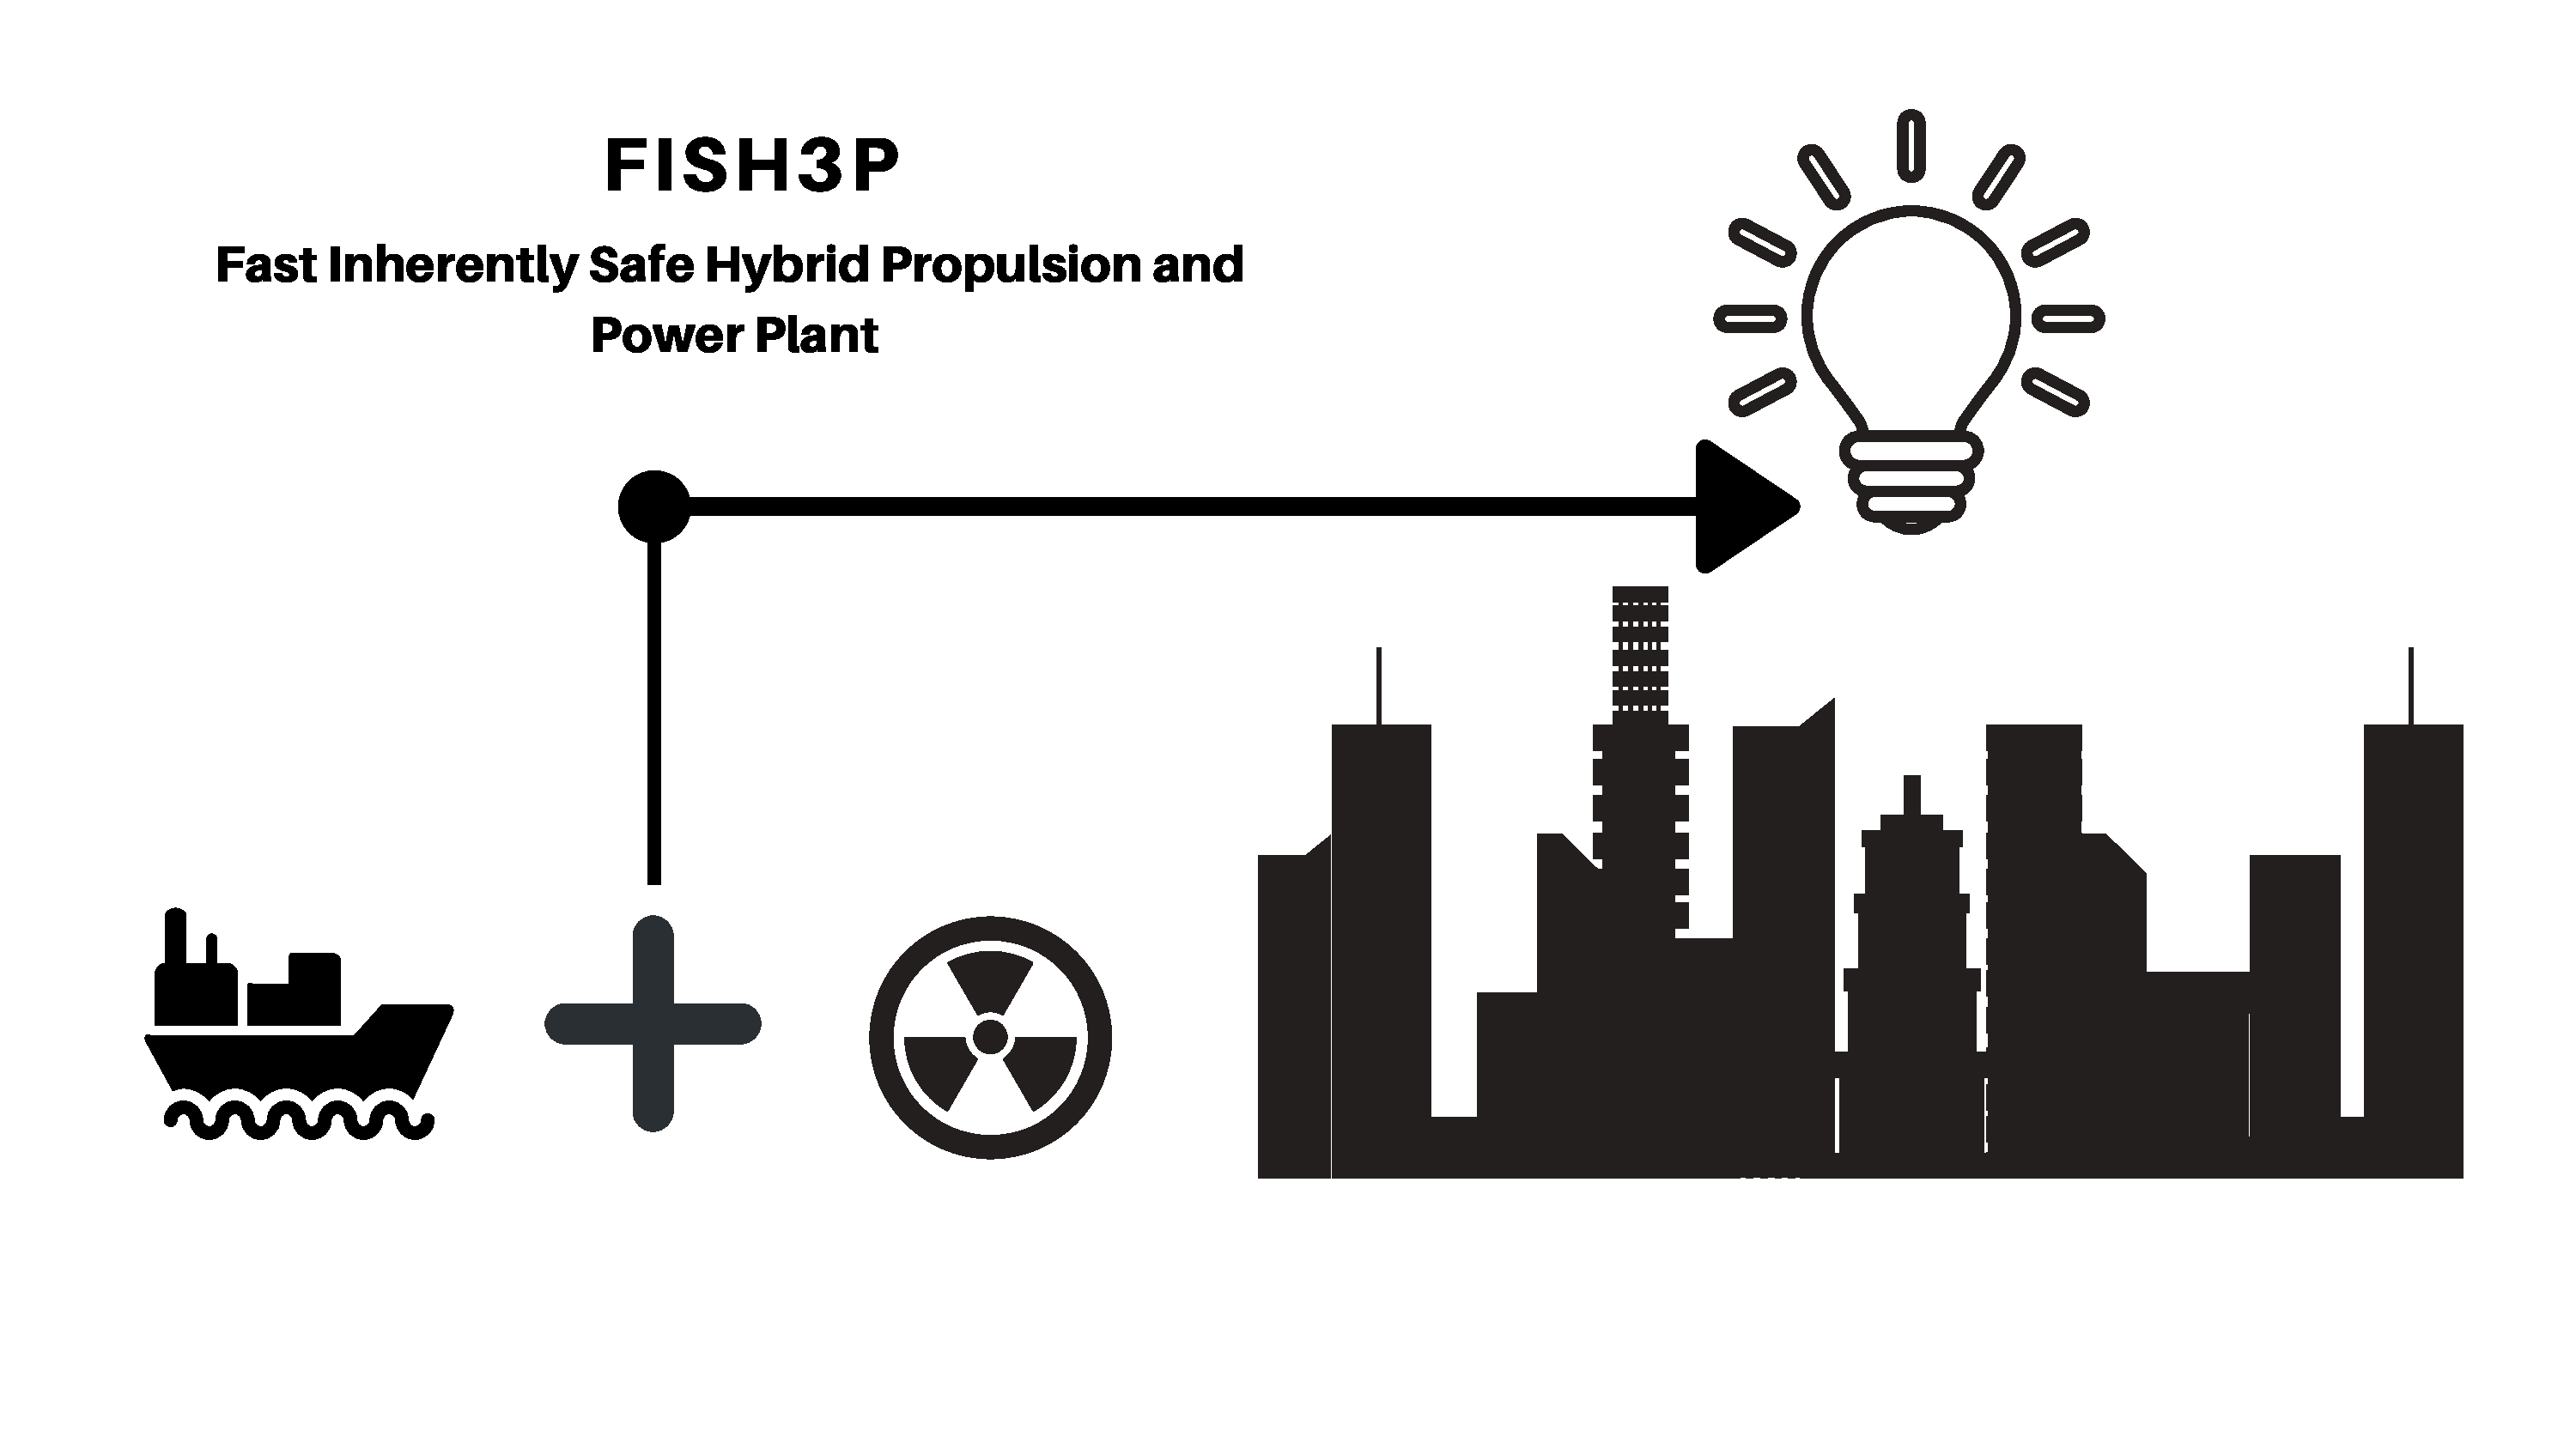
\includegraphics[width=1\textwidth]{design_logo}   
    \label{fig:mesh1}     
\end{figure}   
%
\pagebreak
%ABSTRACT
\begin{abstract}
FISHP$_3$ stands for ''Fast Inherently-Safe Hybrid Propulsion and Power Plant". This name reflects every aspect of the proposed design concept. The reactor concept is a driven system derived from a proposition from Ragheb \cite{ragheb_pres}. This system is composed of a pair of annular cylinders, which we refer to as the inner and outer cores. The outer core will be higher in enrichment but lower in volume and power, while the inner core has a larger enrichment but is subcritical. The outer core will thus drive the reaction in the inner core. The outer core is designed as a pebble bed, allowing it to drain away from the inner core and lose criticality if it is not actively powered. We seek to couple this neutronic safety achieved by the novelty of the design with enhanced thermal safety by operating the reactor at sea so that it is placed in the largest possible heatsink. The marine setting of this system allows us to penetrate the shipping market and/or offshore generation of electricity. This report describes the concept in greater detail and provides very simple calculations to demonstrate its feasibility. Additionally, we have written a detailed market analysis and we have identified the constraints that will define our design going forward. Finally, the report contains several diagrams that were created as part of our process planning exercises, including SWOT, Fishikawa, and GANTT diagrams.
\end{abstract} 

\pagebreak
\tableofcontents, 

%\begin{multicols}{2

%%%%%%%%%%%%%%%%%%%%%%%%%%%%%%%%%%%%%%%%%%%%%%%%%%%%%%%%%%%%%%%%%%%%%%%%%%%%%%%%
\section{Introduction}
There are many obstacles to decarbonising a modern economy. Two of these are the Carbon intensity of transportation and the lack of zero-Carbon power that may shutdown during periods of low demand. The solution to both of these problems may lie in nuclear power. We propose a small reactor system with an output on the order of tens of Megawatts that may sell power to the shore during periods of peak electricity demand or use its power for the propulsion of short-range vessels during off-peak hours. 

Offshore nuclear power has advantages beyond its capacity to propel shipping vessels. Namely, these plants are remote from any major population centers, far enough offshore that they do not face risks from tall waves and tsunamis, and their mobility allows them to supply power to remote locations or to cities that have recently survived a natural disaster. Additionally, a plant that sits in the ocean has fantastic thermal safety relative to a terrestrial plant thanks to the infinite heat sink provided by the ocean. To complement this thermal safety we have elected to design a core that achieves the greatest criticality safety possible by designing a subcritical core that is driven by an external neutron source. 

In particular, we imagine an annular assembly in which the inner region is designed such that the infinite multiplication factor $k_\infty = 1$. This passive system will be driven by a source of neutrons blanketed around it. These neutrons will be supplied by an outer core with $k_{eff} = 1 $ 

% If you wanna cite Alekseev put \cite{alekseev}

% If you wanna cite Carlton put \cite{Carlton}

% \cite{Gravina}

% \cite{Han}

% \cite{iaea}

% If you wanna cite Hirdaris put \cite{Hirdaris}

% If you wanna cite Jacobs put \cite{Jacobs}

% If you wanna cite Holtec put \cite{Holtec}

% \cite{heuser_burnup}

% \cite{ragheb_code}

% \cite{ragheb_pres}

% \cite{cyl_derivation}

%%%%%%%%%%%%%%%%%%%%%%%%%%%%%%%%%%%%%%%%%%%%%%%%%%%%%%%%%%%%%%%%%%%%%%%%%%%%%%%%
%%%%%%%%%%%%%%%%%%%%%%%%%%%%%%%%%%%%%%%%%%%%%%%%%%%%%%%%%%%%%%%%%%%%%%%%%%%%%%%
\section{Conceptual Design}
%%%%%%%%%%%%%%%%%%%%%%%%%%%%%%%%%%%%%%%%%%%%%%%%%%%%%%%%%%%%%%%%%%%%%%%%%%%%%%%%
\subsection{Naval concept}
%%%%%%%%%%%%%%%%%%%%%%%%%%%%%%%%%%%%%%%%%%%%%%%%%%%%%%%%%%%%%%%%%%%%%%%%%%%%%%%%
\subsubsection{Nuclear Merchant Shipping Vessels}
%%%%%%%%%%%%%%%%%%%%%%%%%%%%%%%%%%%%%%%%%%%%%%%%%%%%%%%%%%%%%%%%%%%%%%%%%%%%%%%%
Nuclear shipping vessels for commercial use are not a new concept.  Three ships have been built solely for the purpose of commercial shipping of materials.  These designs and their purposes can be seen in Table 1.

\begin{table}[H]
\begin{center}
\caption{Descriptions of the Four Nuclear Merchant Vessels \cite{historic_ships}}
\label{t:KLT-40S2}  %%SHORT AND MEMORABLE LABEL
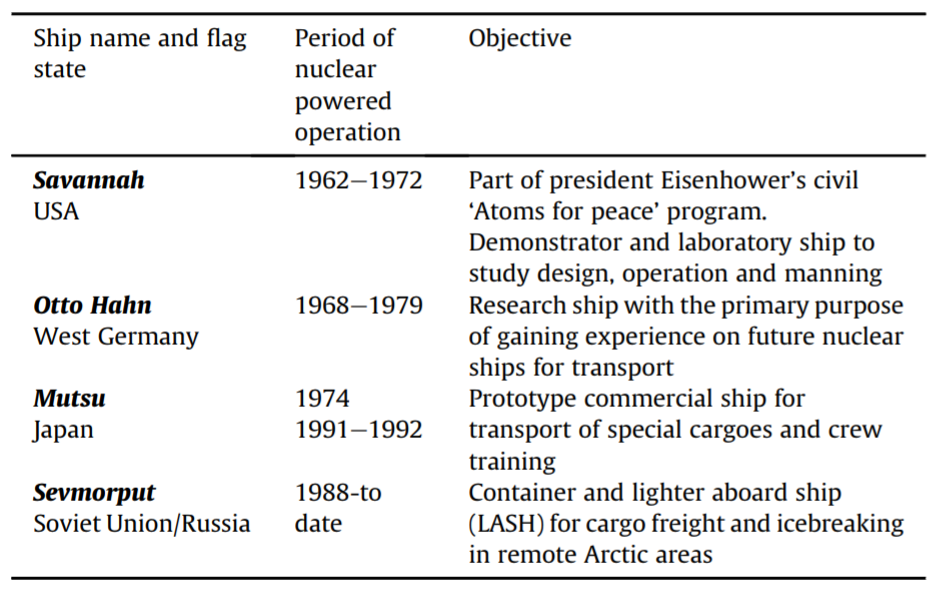
\includegraphics[width=0.85\textwidth]{four_ships} %NAME OF FILE WITHOUT EXTENSION
\end{center}
\end{table}

The lessons learned from these ships are described so that the FISH3P design learns from these mistakes.

\begin{enumerate}
\item \textbf{Savannah}: \newline
In ten years, this vessel traveled to countries across the world, excluding Australia, New Zealand, and Japan.  It was an important step for public opinion on nuclear-powered commercial ships and provided valuable information on marine refueling of the reactor.  However, the ship was not economic as a cargo ship.  
\item \textbf{Otto Hahn}: \newline
Each refueling of this ship required approximately 10 weeks, which is not ideal for a merchant vessel.  Clearance could not be obtained from the port authorities when it docked, making the Otto Hahn unable to complete its cargo shipments.  Because of its inability to receive clearance, its reactor was decommissioned and replaced with a diesel engine.  
\item \textbf{Mutsu}: \newline
During one of its voyages, the Mutsu began to leak fast neutrons.  This leak caused protest from the local inhabitants because of the increased exposure and dose.  These protests were successful in denying access for the ship to be returned to its home port.  Without public communication, trust, and sufficient technical design, the reactor was replaced with a diesel engine and still operates today.
\item \textbf{Sevmorput}: \newline
After the Chernobyl accident, this Russian ship was denied access to ports in the eastern region of Soviet Russia.  It was able to find a route that would accept it to dock, the Muramsk-Dudinka route, after being docked for almost 10 years.  This ship has been able to move cargo through the icy waters for several years without any major accidents. 
\item \textbf{FISH3P}: \newline
The lessons learned from these ships can be described as economic in the case of Savannah, technological in the case of Otto Hahn and Mutsu, and political in the case of Sevmorput.  The FISH3P reactor intends to minimize these types of problems so that it can ship without major issue.  Building public trust is an important aspect of any nuclear design because the public has a generally cautious view of nuclear power.  Creating proactive instead of reactive regulations on commercial nuclear shipping would help reduce these fears.  In the past, regulations on nuclear shipping vessels were created in response to accident.  These regulations from the IMO and NRC on ships like the FISH3P would make it possible port entry into a variety of ports across the world.  The refueling issue of the Otto Hahn could be minimized in the FISH3P design by including a molten salt or pebble-fuel surrounding the inner reactor core.  These fuels allow for online refueling which would increase the amount of time the ship can spend on the sea.  The technological problems of the Mutsu will be minimized by utilizing an inherently safe reactor design, which can shut down in the case of fast neutron leakage.  Providing sufficient biological shielding for the reactor will also reduce the likelihood of this scenario.

\end{enumerate}



%%%%%%%%%%%%%%%%%%%%%%%%%%%%%%%%%%%%%%%%%%%%%%%%%%%%%%%%%%%%%%%%%%%%%%%%%%%%%%%%
\subsubsection{Floating Nuclear Power Plants}
%%%%%%%%%%%%%%%%%%%%%%%%%%%%%%%%%%%%%%%%%%%%%%%%%%%%%%%%%%%%%%%%%%%%%%%%%%%%%%%%
The concept of naval nuclear power expands even further past nuclear submarines, aircraft carriers, and nuclear shipping vessels. A considerable amount of research has also been dedicated towards the design of floating ocean nuclear power plants. There are quite a few advantages to this new concept, most of which correlate directly to its operation at sea instead of on land. First of all, with the nuclear plant residing at sea, there is no longer an issue in locating or acquiring new land for the nuclear plant to occupy for 40 to 70 years. Moreover, the general negative public feedback of nuclear power becomes much less of a factor as the ocean nuclear power plant is out of sight and out of mind in the public’s eye. In this sense, the planning, siting, licensing, and implementation of a new reactor becomes much less of an issue, allowing for a much speedier deployment process as more of a focus can be placed on the physical construction of the plant. Additionally, as this is a floating nuclear reactor without a fixed location, it also acts as a mobile power source, having the ability to be stationed anywhere along the coast as needed. This can be particularly beneficial in providing electricity for large areas with low human populations, or for certain areas experiencing a shortage of power for an extended period of time. The final and perhaps most notable of the advantages for a floating nuclear reactor is in its regard to safety, as the nuclear plant is farther away from the human population when it is at sea. On the off-chance a nuclear accident was ever to occur within the reactor, the ramifications of the fallout from such a nuclear disaster could be minimized through its increased distance from human life. Furthermore, the open ocean provides these types of reactors with an endless supply of cooling water if an accident were ever to occur.

\begin{itemize}

    \item \textbf{Akademic Lomonosov}
    
    Russia has done quite a bit of work in this area of naval nuclear designs as well, beginning construction of the first ocean nuclear power plant in 2007. This floating nuclear power station, known as the Akademik Lomonosov, became operational in December 2018. A particularly exiting aspect of this design is the fact that it can also be used as a desalination plant for developing countries with a low water supply. It uses two KLT-40S pressurized water reactors, each capable of producing up to 35 MW of electricity with 150 MW of thermal power. These reactors have been specifically designed to use uranium fuel consisting of a U-235 enrichment of 14.1\%. This is within the 20\% enrichment limit for Low-Enriched Uranium (LEU) set by the IAEA, which is stated to promote proliferation resistance. The main characteristics and parameters of the KLT-40S reactor are defined within Table \ref{t:KLT-40S1} and Table \ref{t:KLT-40S2}, respectively. The Akademik Lomonosov is 144 meters long and 30 meters wide, with a displacement of 21,500 tons. The crew to operate this station expands to about 70 people. The plant is projected to be operational for 40 years, with refueling occurring every 3 years. \cite{ONPP}
    
    \begin{table}[H]
    \begin{center}
     \caption{Main characteristics of each KLT-40S reactor within Akademic Lomonosov \cite{KLT}} %%DESCRIPTIVE CAPTION
     \label{t:KLT-40S1}  %%SHORT AND MEMORABLE LABEL
     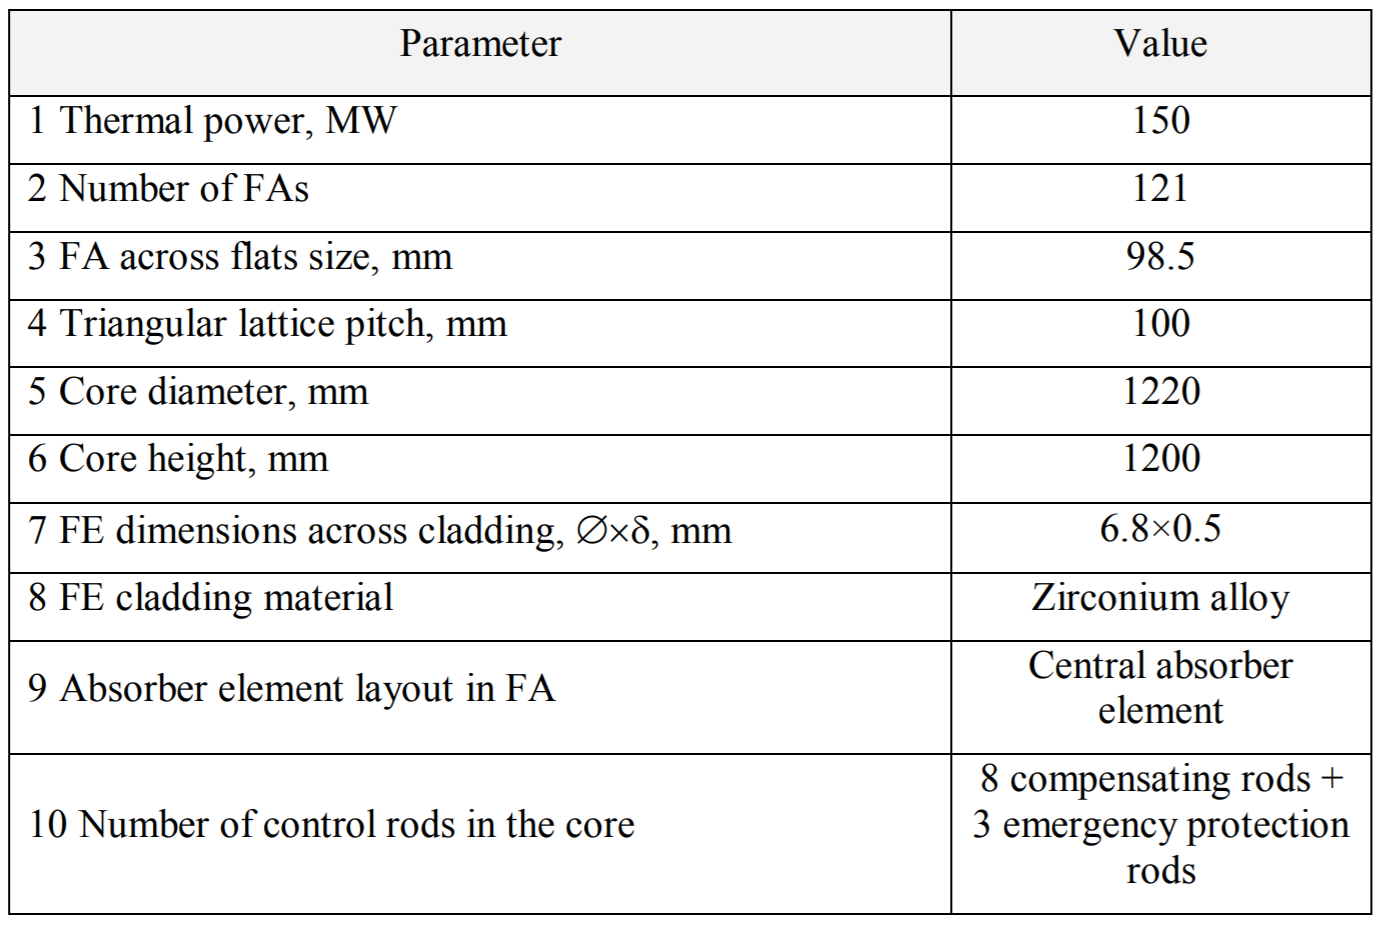
\includegraphics[width=0.85\textwidth]{KLT-40S1} %NAME OF FILE WITHOUT EXTENSION
    \end{center}
    \end{table}
    
    \begin{table}[H]
    \begin{center}
     \caption{Main parameters of each KLT-40S reactor within Akademic Lomonosov \cite{KLT}} %%DESCRIPTIVE CAPTION
     \label{t:KLT-40S2}  %%SHORT AND MEMORABLE LABEL
     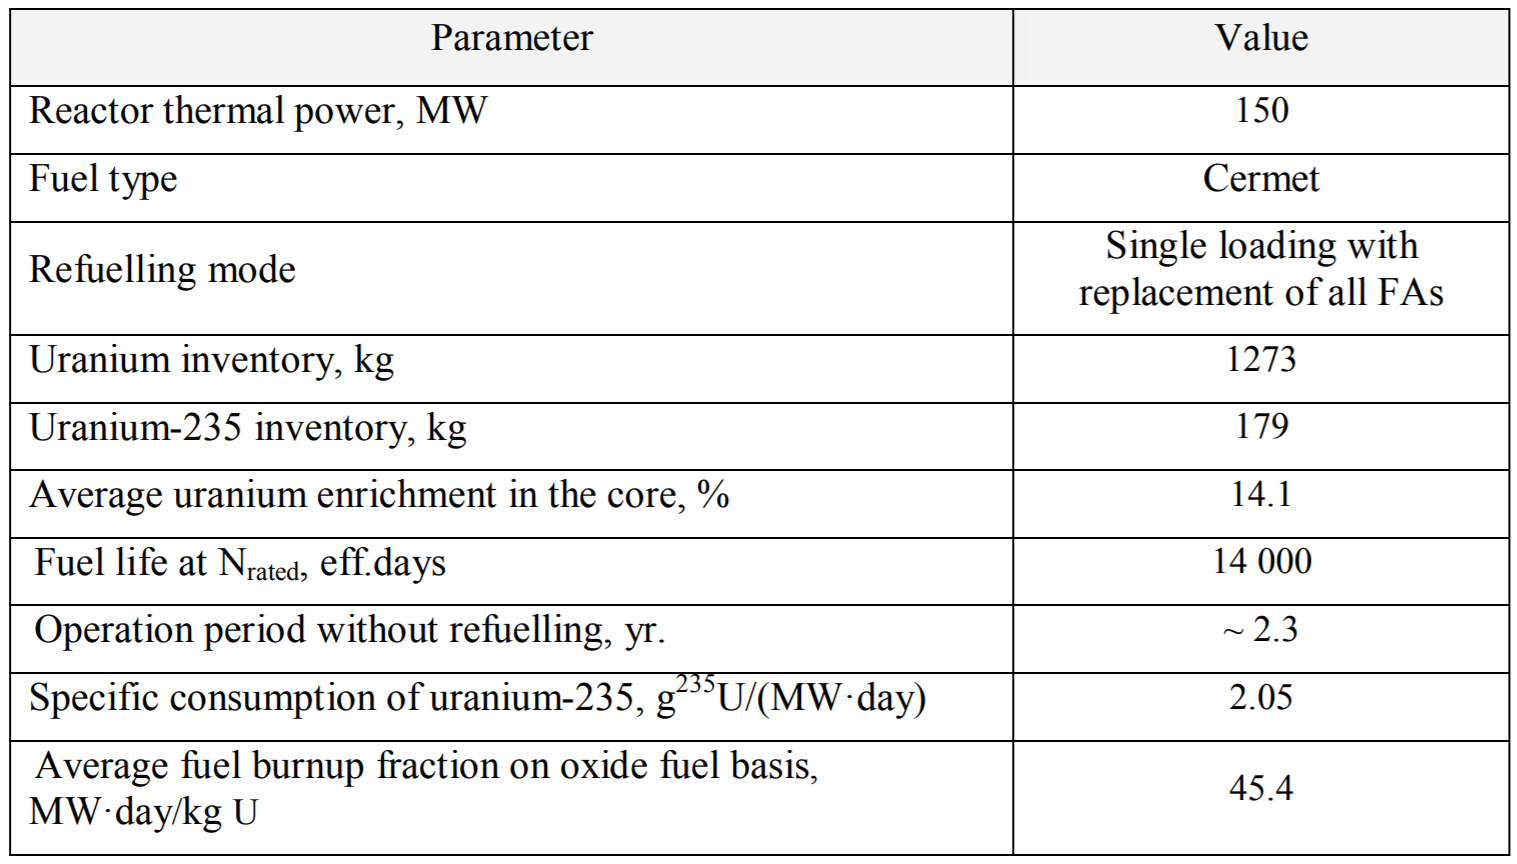
\includegraphics[width=0.85\textwidth]{KLT-40S2} %NAME OF FILE WITHOUT EXTENSION
    \end{center}
    \end{table}
    
    \item \textbf{Offshore Floating Power Plant (OFNP)}
    
    In June 2015, a research group in the Nuclear Science and Engineering Department of the Massachusetts Institute of Technology proposed a new design for an Offshore Floating Nuclear Plant. Unlike the Akademic Lomonosov, this power plant is designed to produce either 300 or 1100 MW of electricity—a much greater feat than the Russians, if ever operational. The OFNP300 is designed largely around the Westinghouse Small Modular Reactor (WSMR), and is set to be about 73 meters tall, 45 meters in diameter, and have a displacement of 115,500 tons. The OFNP1100 is designed around the AP1000 reactor, and is set to be about 108 meters tall, 75 meters in diameter, and have a displacement of 376,400 tons \cite{OFNP}. The designs for the OFNP300 and OFNP1100 are illustrated in Figure \ref{fig:OFNP300} and Figure \ref{fig:OFNP1100}, respectively.  Instead of being located right at the shore line like the Akademik Lomonosov, the OFNP is designed to reside 8 to 12 miles out at sea, in water about 100 meters deep. There are quite a few benefits to this design aspect. First of all, the reactor will be much farther from coastal populations. Moreover, the great depth of water underneath the reactor and its increased distance from the shore will reduce any potential threats caused by earthquakes or tsunamis. This is due to the fact that tsunamis have a much smaller amplitude further out to sea, and only rise in height as it approaches the shoreline. Therefore, tsunamis truly only become destructive near the shore, which was the primary cause of the Fukushima Daiichi nuclear disaster. This is the exact situation this offshore floating nuclear plant is designed to counteract. 
    
    \begin{figure}[H]                                  
        \centering                                     
        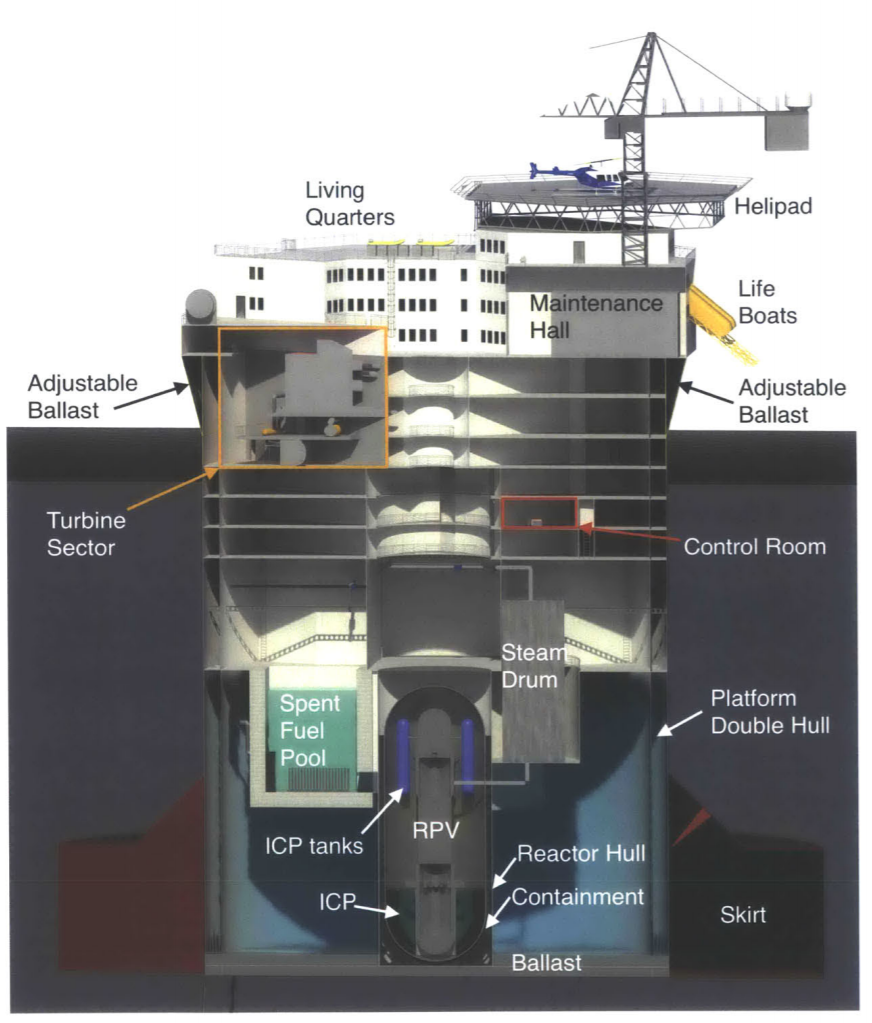
\includegraphics[width=\textwidth]{OFNP300}   
        \caption{Cross Section of OFNP300}
        \label{fig:OFNP300}     
    \end{figure}
    
    \begin{figure}[H]                                  
        \centering                                     
        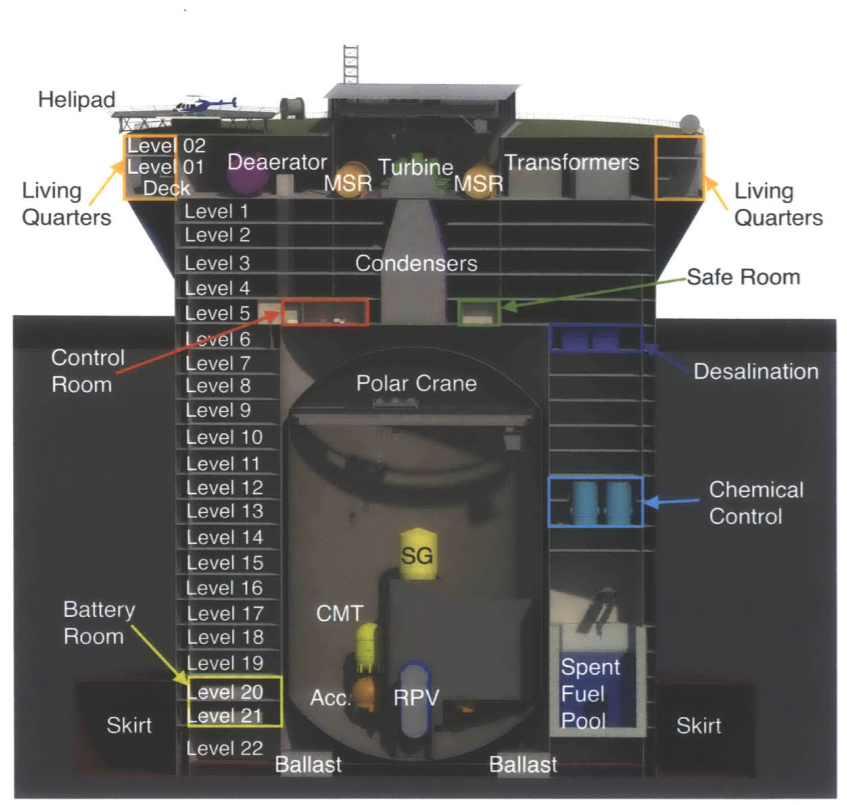
\includegraphics[width=\textwidth]{OFNP1100}   
        \caption{Cross Section of OFNP1100}
        \label{fig:OFNP1100}     
    \end{figure}
    
\end{itemize}

%%%%%%%%%%%%%%%%%%%%%%%%%%%%%%%%%%%%%%%%%%%%%%%%%%%%%%%%%%%%%%%%%%%%%%%%%%%%%%%%
\subsection{Reactor concept}
%%%%%%%%%%%%%%%%%%%%%%%%%%%%%%%%%%%%%%%%%%%%%%%%%%%%%%%%%%%%%%%%%%%%%%%%%%%%%%%%
\subsubsection{Driven Reactor}
%%%%%%%%%%%%%%%%%%%%%%%%%%%%%%%%%%%%
The FISHP$_3$ reactor achieves its namesake inherent safety by surrounding a subcritical core with an annular critical core. The majority of the power is generated in the inner core, which is designed such that the infinite multiplication factor $k_\infty$ remains at unity. This property will ensure a flat flux profile in the inner core. The outer core will be fueled by high assay low enrichment Uranium fuel such that its effective multiplication factor $k_{eff}$ is unity. We imagine that this Uranium will be in the form of a fluidized pebble bed such that if power is lost, these pebbles will drain from the core into a suppression pool with a less critical geometry. This design will ensure that the entire reaction will shut down when power is not actively supplied to the outer core. Additionally, the placement of the reactor over the water provides an infinitely large ultimate heatsink, ensuring the thermal safety of the system.

Because the reactor geometry will be cylindrical, this will lead to a flux profile described by a flat region in the interior and a Bessel function in the outer region. Such a flux profile is depicted in \ref{f:standing-wave}. The flatness of this region guarantees even burnup in the inner core, which provides a great cost savings 

\begin{figure}[H]                                  
    \centering                                     
    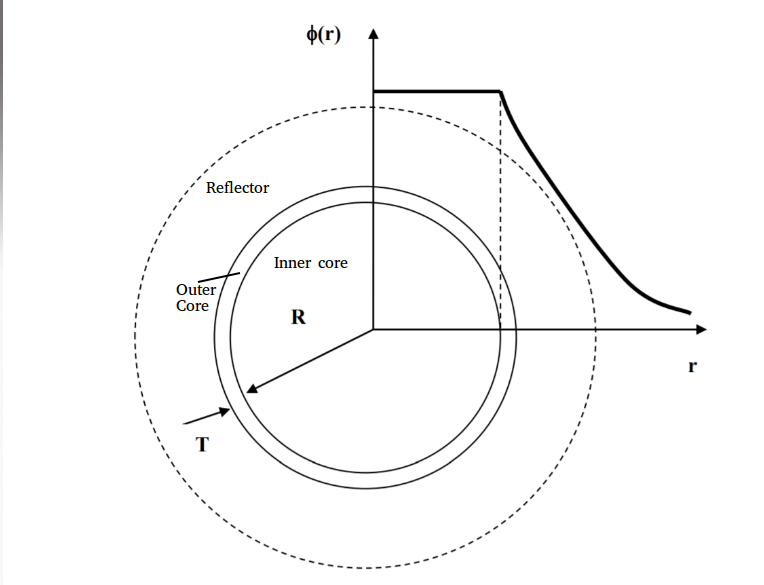
\includegraphics[width=0.69\textwidth]{standing-wave}   
    \caption{A sketch of the proposed reactor system}                          
    \label{f:standing-wave}     
\end{figure}     

However, this concept is not without its weaknesses. To maintain the uniform flux profile, it is necessary to design the reactor to operate on the fast end of the neutron energy spectrum, which requires a greater enrichment in $^{235}U$ than a thermal reactor. Additionally, it is difficult to design a control system for a fast reactor because most neutron poisons (such as Boron-10 and Xenon-135) prefer to capture thermal neutrons. Fast reactors typically must rely on Doppler Broadening in the fuel to maintain criticality control \cite{ebr2}.

There are numerous other reactor concepts that may better fit our design goals. Although our preference is with the driven ``standing wave" design discussed above, brief discussions of the merits and drawbacks of other reactor concepts is available in the following subsection.

\subsubsection{Alternatives}
\begin{enumerate}
    \item \textbf{Fast-spectrum metal-cooled reactor}: The driven system may prove too difficult or impractical to design, in which case it may be simplest to design a critical system with a metal coolant. However, many other disadvantages of the driven system would remain such as the corrosivity of the coolant and the large power required by the coolant pump.
    \item \textbf{High-temperature gas cooled reactor}: The HTGR provides another option in the world of fast reactors that also offers excellent Carnot efficiency. However, these systems require a very low power density which is poorly suited for a marine application.
    \item \textbf{Molten salt reactor}: An MSR has many advantages. Particularly, this system may refuel and reprocess online, negating any Xenon dead-time. This opportunity would be invaluable in a propulsion system that must increase and decrease power frequently. However, the chemical facilities to perform this reprocessing would be difficult to fit onto a boat. The molten salt system would also come with concerns regarding corrosion and reactivity with water.
    \item \textbf{Light Water Reactor}: An LWR design has the most operational history in both marine and terrestrial contexts. These designs are the most natural and straightforward in this context. However, they require high enrichment to overcome Xenon poisoning and to scale down to appropriate sizes. Additionally, the coolant is reactive with Zirconium at high temperatures, exacerbating disaster scenarios.
\end{enumerate}

%%%%%%%%%%%%%%%%%%%%%%%%%%%%%%%%%%%%%%%%%%%%%%%%%%%%%%%%%%%%%%%%%%%%%%%%%%%%%%%%
\section{Feasibility analysis}
\subsection{Ship analysis}
\subsubsection{Safety}

\item \textbf{Previous Design Considerations}: \newline
An important concept to consider when designing safety mechanisms for a nuclear-powered vessel is the strengthening of materials surrounding the nuclear plant so that it is not penetrated in the event of an accident.  The Otto Hahn achieved this goal by creating cutting decks that would penetrate the colliding object.  This effectively reduced the impact penetration of the colliding object and the ship.  If an accident were to take place, the liquid outer core would no longer surround the inner core, resulting in a subcritical system.  Only decay heat from the inner core and from the container where the now-solid molten salt drained.  Creating a sandwich material consisting of “Y” frames could also achieve this goal by absorbing much of the impact energy.  To absorb more energy, these “Y” structures are built from material that fails in a ductile manner.  Stranding, or leaving the boat on the shore, could also pose problems for the reactor because of the force balance.  This problem can be avoided by placing the reactor on a pedestal with rupture discs in the connecting pipes in case of large forces or moments on the reactor.  If the vessel were to sink for any reason, the reactor compartment must be able to handle the pressure buildup associated with the environment.  Terrorism must also be considered for any reactor expecting operation in the future.  This is a different type of problem because terrorism can be carried out in many ways, but this effect can be mitigated by the inherent safety design criteria utilized by the FISH3P.  If the safety systems are passive and do not require operator control, it is unlikely that terrorism can have a significant impact in the short term.  Having alarms so that communication between the ship and the nearby shore will be implemented into the safety criteria.
\item \textbf{Salvaging the Reactor}: \newline
If a catastrophic event occurs on the ship, causing it to sink, the FISH3P will be designed to handle the high pressures of the ocean.  Ideally, this reactor should able to disconnect from the ship after a certain force is placed on it, allowing it to be salvaged.  This mechanism will be helpful in easing public fears concerning a nuclear accident and reduce environmental damage. Additionally, Jacobs has proposed a system of inflatable plastics that can surround the reactor and give it buoyancy in the case of disaster \cite{Jacobs}.

\item \textbf{Radiation Safety}: \newline
The effects of radiation on man is a complex problem to comprehend because the radiation exposed to a person does not adequately give the picture on what this person absorbed.  Often there is a weighing factor depending on the organ being exposed to a given type of radiation.  Not all radiation affects each part of the body equally; some organs are more vulnerable than others.  Radiation damages healthy issue by releasing energy into the cells, causing mutations or cell death depending on the dose.  Cell tissue is mostly proteins and water, so the radiation will deposit its energy in these molecules to cause cell damage.  The level of damage caused to the cell is determined by the type of radiation, the exposure time, the stage in life for the cell, and other factors. 

\begin{enumerate}
\item \textbf{Exposure}: \newline
Because life evolved with exposure to radiation from the earth and cosmic radiation, this dose is not considered significantly harmless.  However, large exposures of radiation will cause damage which is why permissible levels of exposure and dose have been calculated using previous experiments on animals and people who unfortunately experienced large doses of radiation.  The exposure of radiation is defined as the ionization of air due to ionizing radiation from photons.  Calculations of a cylindrical source will be included soon, however, the exposure rate, F, can be defined as shown in Equation 1.

\begin{align}
F &= \Gamma \times \frac{\alpha}{r^2} 
\end{align}

In Equation 1, F represents the exposure rate, r is the distance from the point source, $\alpha$ is the source activity, and $\Gamma$ is the exposure rate constant determined by the gamma source.  The calculations of exposure for the FISH3P reactor will require shielding be included in this calculation with a cylindrical 

\item \textbf{Absorbed Dose}: \newline
Unlike exposure, absorbed dose measures the amount of radiation deposited in the body of interest by ionizing radiation.  This is an important quantity to radiation safety because not all radiation exposure to the human body is deposited in the tissue.  For example, alpha radiation has a very short range and cannot penetrate the skin.  With such a high stopping power, absorbed dose is calculated from alpha radiation if it is external.  However, if the radiation is internal, the energy will be stored in the tissue.  Because absorbed dose is not uniform in the body, it is calculated as an average weighted by mass of the absorbed doses at each piece.

\begin{align}
D_T &= \frac{\int(D(x,y,z)\rho(x,y,z)dV}{\rho(x,y,z)dV} 
\end{align}

In Equation 2, T is the body, D is the dose as a function of space, and $\rho$ is the density as a function of space.  This calculation will be carried out for the FISH3P reactor, simplifying it as a cylindrical source of radiation in cylindrical coordinates.  The body of interest will be a typical worker.

\item \textbf{Equivalent Dose}: \newline
The equivalent dose represents the health effects of radiation on the human body.  Essentially, 
the absorbed dose at each area of interest is weighed by a factor discussed earlier.  Because not all parts of the body are affected equally by radiation, there must be a weighing factor for the organs that are vulnerable.  The calculation for this dose equivalent is shown in Equation 3.

\begin{align}
H_T &= \sum (W*D_T) 
\end{align}
In Equation 3, H is the equivalent dose, W is the weighing factor, and D is the absorbed dose.

\item \textbf{Limits on Occupational Exposure}: \newline
The U.S. Navy publishes documents concerning the exposure of their nuclear workers and the federal annual and quarterly limits.  Radiation exposure has decreased for Navy workers in spite of an increase in nuclear vessels.  This trend is demonstrated in Figure 4.

\begin{figure}[H]                                  
    \centering                                     
    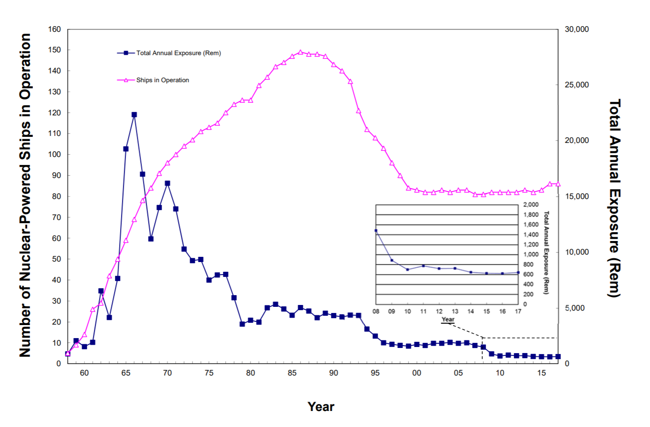
\includegraphics[width=1\textwidth]{exposure-navy}   
    \caption{T annual exposure to workers in REM and the U.S. Navy vessels operational by year}
    \label{fig:mesh1}     \cite{navy_exposure}
\end{figure}       

Since 1967, the exposure limits for the workers has been 3 REM per quarter and 5 REM per year.  1960s there has not been a single civilian for military worker in the Nuclear Naval Propulsion Program exposed to more than 10\% of the annual limit by the reactors.  This indicates that the reactors used in these vessels are quite safe.  It is the goal of the FISH3P reactor design not to exceed 10\% annual limit using their exposure model.  

\end{enumerate}


%%%%%%%%%%%%%%%%%%%%%%%%%%%%%%
\subsubsection{Propulsion}

There is a finite range of container vessels which could utilize a power output of roughly 60 MW from the proposed small nuclear reactor system. The types of ships which need a propulsion power at this level ranges from mid-size to large-size container ships. With the primary objective of this design project seeking to minimize the carbon emissions produced by naval vessels, a larger ship would prove to be more effective and efficient in achieving this goal. With larger nuclear merchant ships come greater shipping capacities, which alleviates the amount oil fueled merchant ships necessary for naval shipping. The charts below show the various sizes, speeds and propulsion of the main types of ships which could utilize the power provided by this type of nuclear naval reactor. As one can see from these figures, with each additional twenty-foot equivalent unit, or TEU, a ship can hold, the more power it will need to move the additional weight.

\begin{figure}[H]                                  
    \centering                                     
    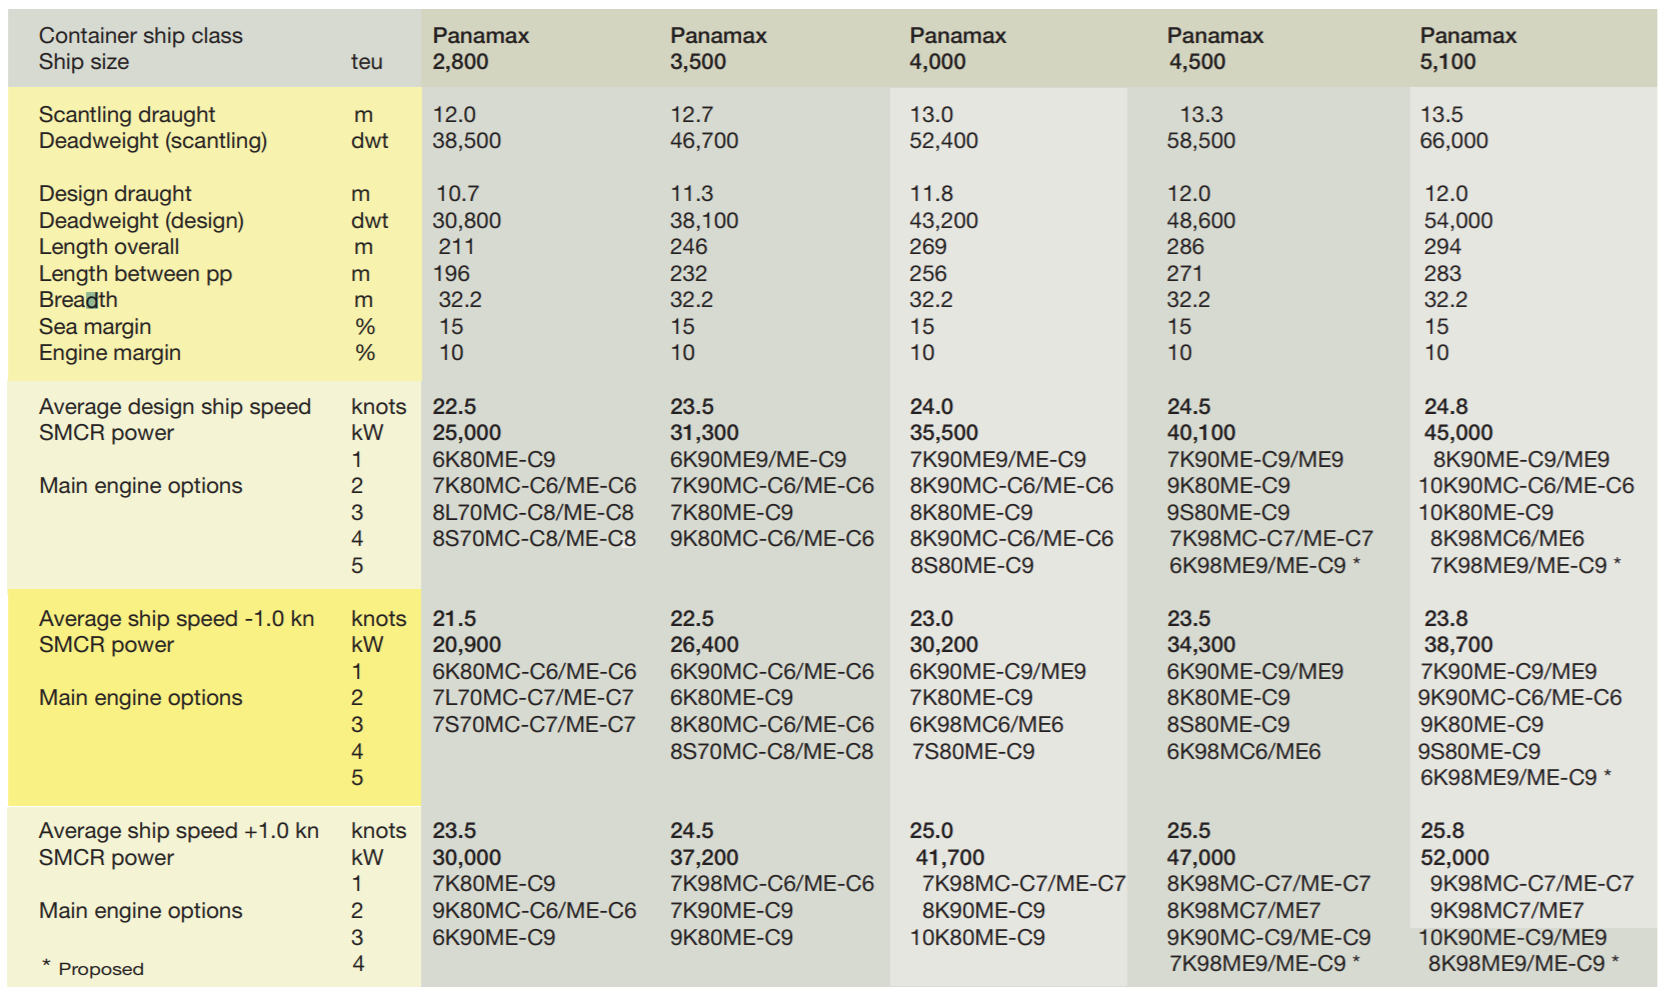
\includegraphics[width=\textwidth]{PropulsionPanamax}
    \caption{Ship parameters and propulsion for Panamax container vessels \cite{propul}}     
    \label{fig:1ship}     
\end{figure}

\begin{figure}[H]                                  
    \centering                                     
    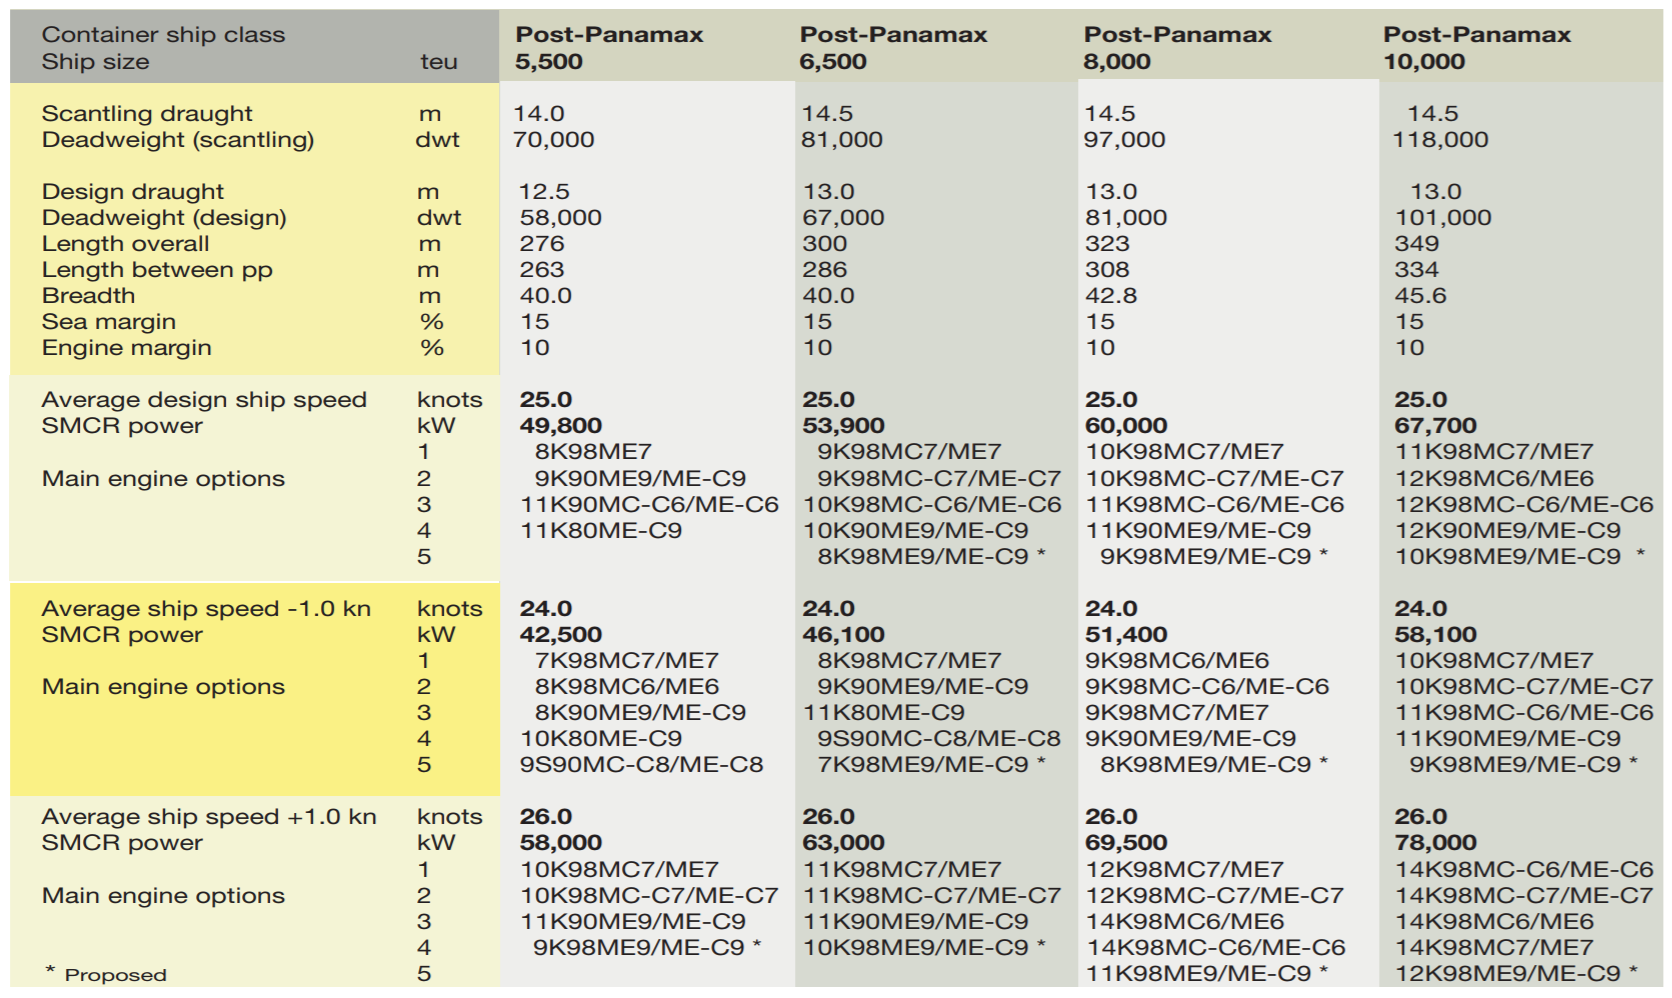
\includegraphics[width=\textwidth]{PropulsionPostPanamax}
    \caption{Ship parameters and propulsion for Post-Panamax container vessels \cite{propul}}     
    \label{fig:2ship}     
\end{figure}

\begin{figure}[H]                                  
    \centering                                     
    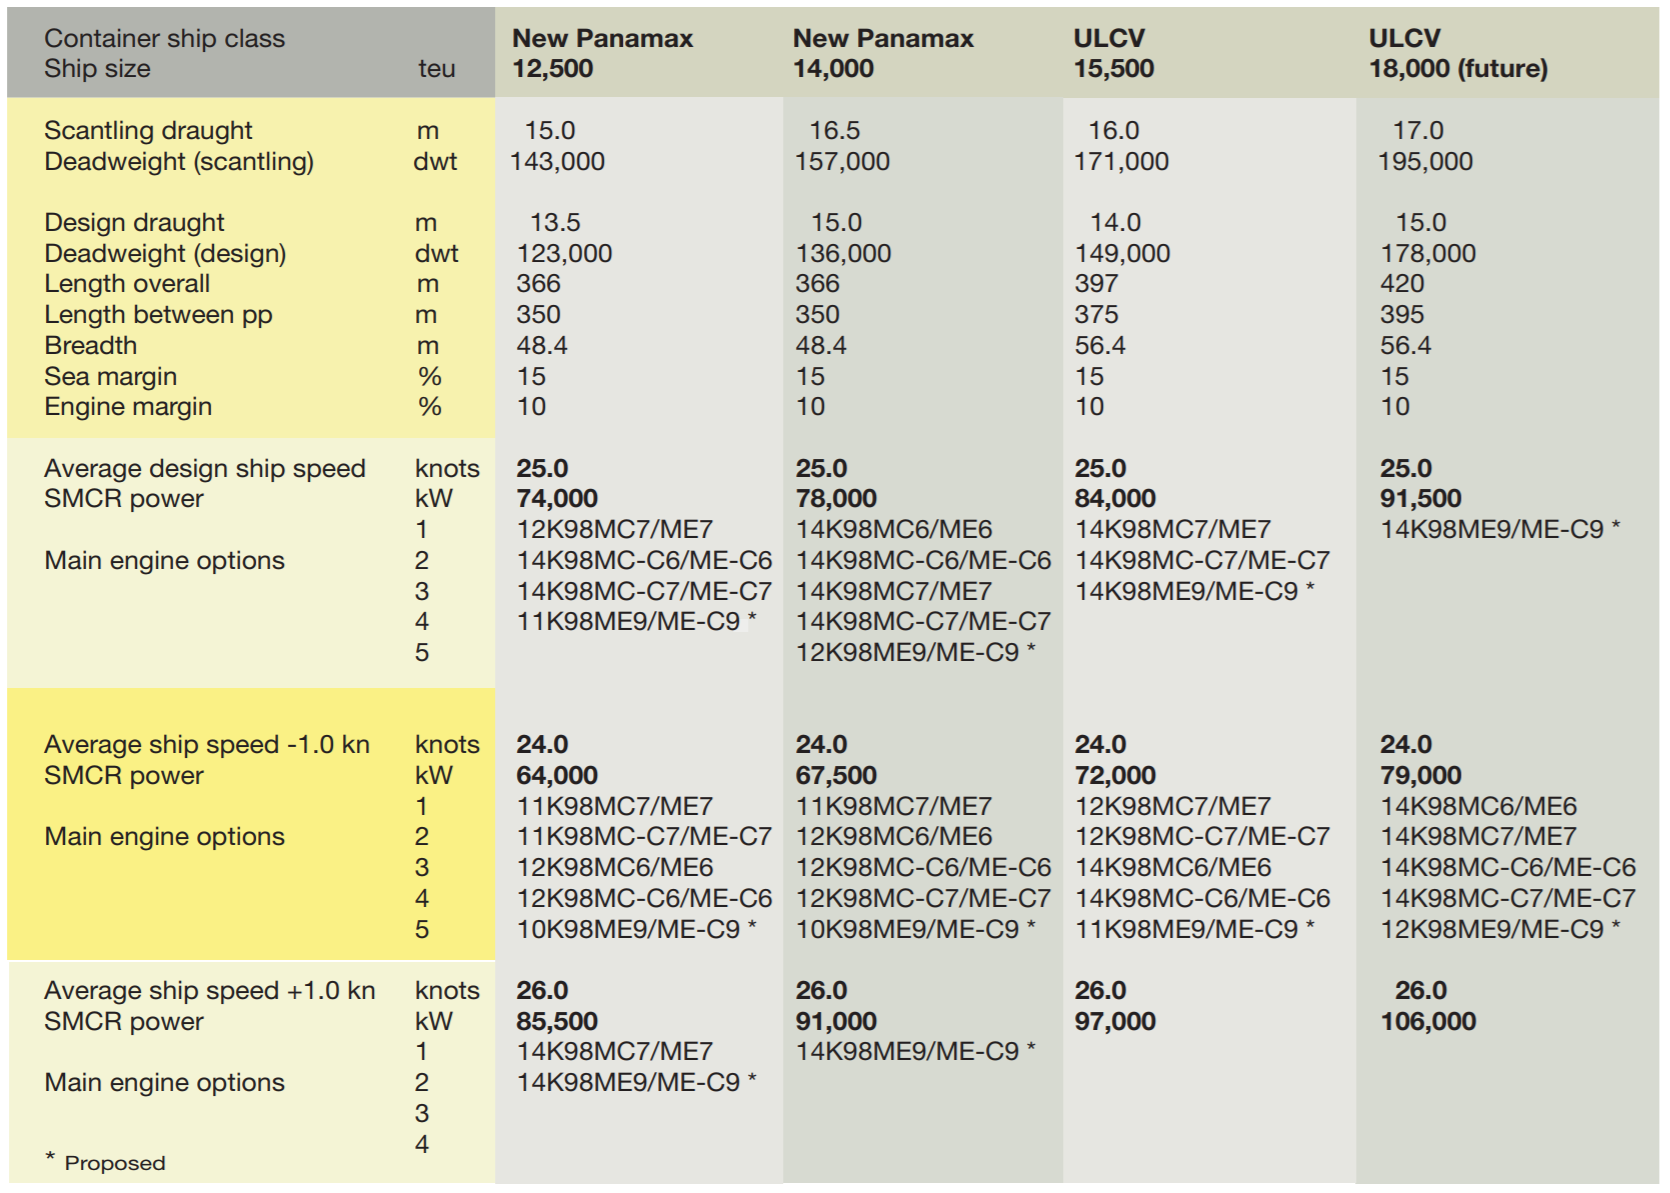
\includegraphics[width=\textwidth]{PropulsionULCV}   
    \caption{Ship parameters and propulsion for New Panamax and ULCV container vessels \cite{propul}}
    \label{fig:3ship}     
\end{figure}

This data is plotted in Figure \ref{fig:graphship} in order to visualize the trend of the increase in necessary power needed as the size of the ship is increased.

\begin{figure}[H]                                  
    \centering                                     
    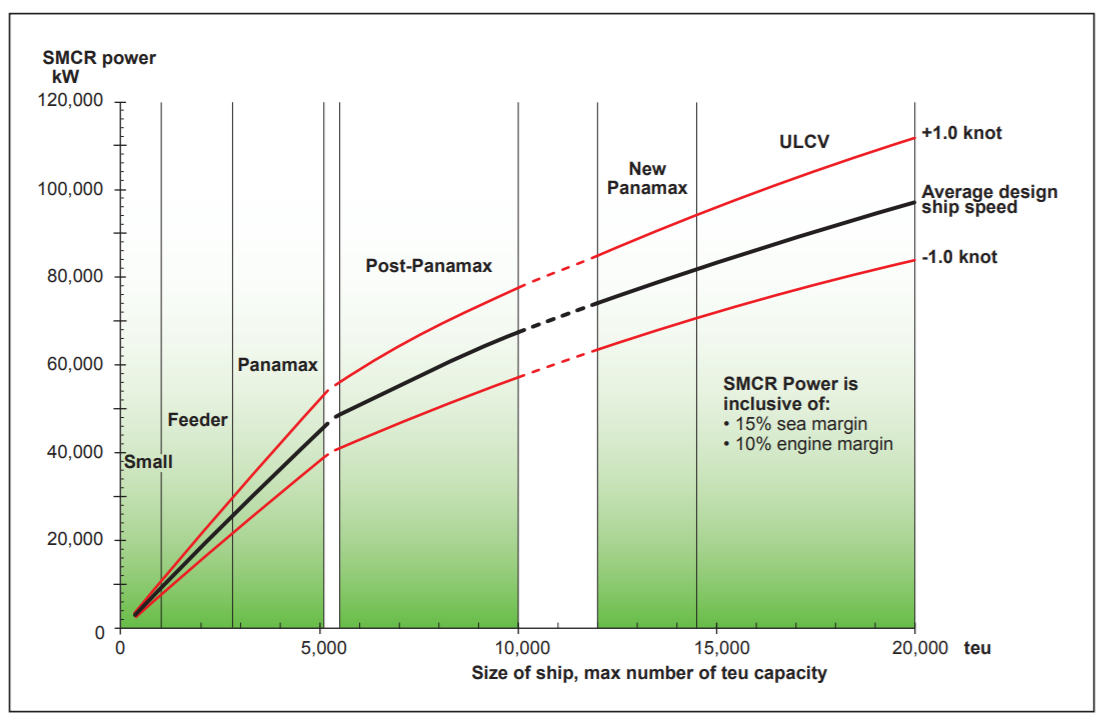
\includegraphics[width=\textwidth]{PropulsionGraph}   
    \caption{Propulsion demand of a container vessel \cite{propul}}
    \label{fig:graphship}     
\end{figure}


%%%%%%%%%%%%%%%%%%%%%%%%%%%%%%%%%%%%%%%%%%%%%%%%%%%%%%%%%%%%
\subsection{Reactor analysis}
Brief back-of-the-napkin style calculations are presented to determine the rough dimensions of the fuel and coolant systems. 
%%%%%%%%%%%%%%%%%%%%%%%%%%%%%%
\subsubsection{Inner core fuel parameters}
The following analysis determines the enrichment required to reach $k_\infty = 1$:

\begin{align}
k_\infty &= \eta f = 1 \\
 &= \nu \frac{\sigma_f^F}{\sigma_a^F} \frac{\Sigma_a^F}{\Sigma_a} \label{e:kinfty}
\end{align}

Approximate values of these parameters are given in table \ref{t:jaea-table}.

\begin{table}[H]
\begin{center}
  \caption{Approximate values of nuclear properties germaine to equation \ref{e:kinfty}, \cite{wirtz}}
  \label{t:jaea-table}
  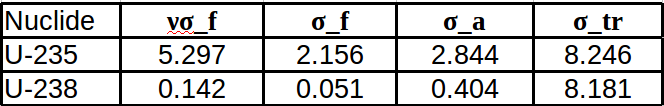
\includegraphics[width=\textwidth]{cross-sections}
\end{center}
\end{table}


The macroscopic cross section is by definition $\Sigma = N \sigma = \frac{\rho N_{av}}{A} \omega$. Equation \ref{e:kinfty} then reduces to:

\begin{align}
1 &= \nu \frac{^{235}\sigma_f}{^{235}\sigma_a} \frac{\frac{\omega}{235} ^{235} \sigma_a}{\frac{1 - \omega}{238} ^{238} \sigma_a + \frac{\omega}{235} ^{235} \sigma_a} \\
 &= \nu \frac{^{235} \sigma_f}{^{238} \sigma_a} \frac{238 \omega}{235 (1 - \omega)} 
\end{align}

This equation may be solved for $\omega$ rather easily, obtaining a numerical value of 4.67 \% with the data in table \ref{t:jaea-table}. 

If the fuel is $UO_2$, then the mass of Uranium per mass of fuel is:

\begin{align}
\frac{m_U}{m_{UO2}} &= \frac{238 (1 - \omega) + 235 \omega}{238 (1 - \omega) + 235 \omega + 32} \\
 &= 0.8814 \frac{grams}{gram}
\end{align}
It is now easy to find the number of $U_{235}$ atoms per gram of fuel:
\begin{align}
n_{235} &= \omega \frac{m_u}{m_{UO_2}} \frac{N_{av}}{235} \\
 &= 1.055 \times 10^{20}
\end{align}

%If we \textbf{assume that $\frac{3}{4}$ of the fissions occur in $U_{235}$}, then the total fissile atoms per gram of fuel is $1.05 \times 10^{22}$. 

We can now determine the required mass of Uranium to produce a certain amount of energy. Knowing that each fission produces $200 MeV = 3.2 \times 10 ^ {-11}$ Joules. Knowing the number of $U_{235}$ atoms per gram of fuel to be $1.063 \times 10^{20}$, we can conclude that each gram of fuel will supply $3.2 \times 10 ^ {-11} \times 1.063 \times 10^{20} = 3.4 \times 10^9$ Joules. An output of 120-MWe-years would therefore require at least 3705 kg of fuel, assuming a thermal efficiency of 30 \%. 

The volume of $UO_2$ that corresponds to this mass is 0.338 cubic meters. We will assume that the volume of our cylindrical core is equal to the volume of a sphere of the same radius, which is to say $H = \frac{4}{3} R$. Under this assumption, the radius of our core is $(\frac{3}{4} \pi V) ^ {1/3} = 0.432 meters,$ giving a height of $0.58 meters$. This first estimate of the height (which will most likely be shorter than the final value) will be very useful in the thermal analysis.

%%%%%%%%%%%%%%%%%%%%%%%%%%%%%%
\subsubsection{Outer core fuel parameters}
Lamarsh gives the Buckling in a finite cylinder as $B^2 = \frac{2.405}{R}^2 + \frac{\pi}{H}^2 = \frac{\nu \Sigma_f - \Sigma_a}{D}$. This should well-approximate the outer core even in the two-region problem, so we can use this equation to estimate the critical thickness of the outer core. We will again assume that the height is 4/3 the radius. The radius is then related to the material properties of the core by the following equations:

\begin{align}
\frac{\nu \Sigma_f - \Sigma_a}{D} &=(\frac{2.405}{R})^2 + (\frac{\pi}{4/3 R})^2 \\
 &= \frac{2.405^2 + \frac{9}{16}\pi^2}{R^2} \\
R &= \sqrt{\frac{2.405^2 + \frac{9}{16}\pi^2} {\frac{\nu \Sigma_f - \Sigma_a}{D}}} \label{eq:outer-radius}
\end{align}

There are multiple sources of error in this estimate of the critical radius. The radial eigenvalue of 2.405 is suspicious because this geometry is not the same as the typical continuous cylinder for which that number was determined. Additionally, the densities used to compute the cross sections in this equation depend on the material type as well as the fuel form. 

However, for simplicity, we will assume a uniform mass of $UO_2$ with density $\rho =  10970 \frac{kg}{m^3}$, as we did in the inner core calculations. We will also assume an enrichment of 19.5 \%, as this is the highest number achievable without using highly enriched fuel. With these conditions, the thickness of the outer core is approximately 70 cm. Compared to the inner core radius determined in the previous subsection, this size is unacceptably large. This flaw may be corrected by increasing the enrichment or the density of the outer core. Increasing the enrichment beyond 20 \% would be a serious sacrifice of our design commitments, so it should be avoided.  There are limited options for denser fuel types. The densest form of Uranium is Uranium metal, which is less than twice the density of the oxide we originally proposed. This choice will almost halve the critical radius of the outer core, but sacrifice the excellent thermal properties offered by the oxide. A more detailed analysis is required to determine the optimal choice in this regard. Another solution would be to simply increase the size of the inner core. Although this would not change the size of the outer core, the fraction of volume in the outer core would fall. Additionally, by increasing the inner core volume we can decrease the flux needed to achieve the same power, which would in turn simplify the cooling of the outer core. 

%%%%%%%%%%%%%%%%%%%%%%%%%%%%%%
\subsubsection{Thermal analysis}
Let us begin by estimating the mass flow rate required to remove the fission heat at steady state. With a simple energy balance, it becomes apparent that heat flux is related to the heat capacity and mass flow rate of the coolant and the temperature change across the length of the channel as follows:

\begin{align}
q &= \dot{m} c_p \Delta T \\
\dot{m} &= \frac{q}{c_p \Delta T}
\end{align}

%We can estimate q'' by dividing the thermal power by the surface area of the fuel, which gives us $q'' = \frac{1.75 \times 10^8}{2 \pi N 0.63 \times 10 ^{-2}}$ if there are N fuel rods, each with 1-cm radius and 1.43 meters tall. For this preliminary analysis, \textbf{we will assume 100 rods}. It then follows that the heat flux from such a system is $4.42 \times 10^7 \frac{w}{cm^2}$. 

Our coolant, Lead-Bismuth Eutectic, is liquid between approximately 200-1670 Degrees C. Neglecting the constraints of other materials, the $\Delta T$ may then approach 1,000 Kelvin. The isobaric heat capacity of this fluid in this temperature range is approximately $130 \frac{J}{kg K}$ \cite{LBE_properties}. 

The Mass flow rate needed to achieve 60 MWe is therefore:

\begin{align}
\dot{m} &= \frac{q}{c_p \Delta T} \\
 &= \frac{200 \times 10^6 \frac{J}{s}}{130 \frac{J}{kg K} \times 10^3 K} \\
 &= 340 \frac{kg}{s}
\end{align} 

Dividing this flow rate by the density of LBE (approximately 9000 kg/m3) gives an approximate volumetric flow rate of 0.038 $\frac{m^3}{s}$, which is roughly one tenth of the volume of the inner core fuel.

However, the temperature difference selected is probably infeasible, as stress corrosion cracking will destroy most materials in this environment at this temperature. We may in fact achieve a temperature difference less than 500 Kelvin, in which case the coolant flow rate required would more than double. Additionally, we may face additional challenges cooling the outer core. In both cases, the problem is simplified by decreasing the power density of the system. 

\subsection{Materials analysis}
To accurately create an analysis of material design, several factors must be analyzed individually.  Included in this materials analysis is the coolant, fuel, cladding, control, shielding, corrosion and radiation damage.  Each factor is compared to potential other materials where appropriate.
\subsubsection{Coolant}
Many coolants are proposed for the FISH3P reactor. Their material properties are discussed in detail here.
\begin{enumerate}
\item \textbf{Lead-Bismuth}:
An optimal coolant for a reactor must contain properties such as a low melting point, high heat capacity, high thermal conductivity, and the primary coolant in the FISH3P reactor was chosen as lead-bismuth eutectic.  This coolant was necessary so that a one-group analysis of the coolant could be achieved and because of its beneficial properties over sodium coolant for the application.  
Lead-bismuth been chosen as an alternative to sodium in this fast reactor design because it eliminates many of the corrosion concerns that liquid sodium presents as a coolant.  Although it has a lower power density, the ship size for this reactor should not pose a concern.  Information concerning the isotopes of lead and bismuth are shown in Table 5 and Table 6 respectively.

\begin{table}[H]
\begin{center}
 \caption{Information concerning the isotopes of lead and their associated energies emitted upon decay} \cite{LBE_properties}
 \label{t:lb-decay}  %%SHORT AND MEMORABLE LABEL
 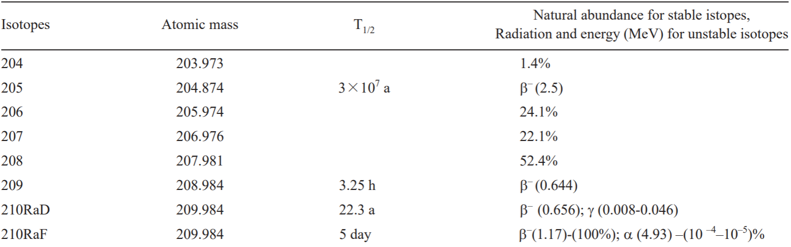
\includegraphics[width=\textwidth]{tab-lb-decay-properties} %NAME OF FILE WITHOUT EXTENSION
\end{center}
\end{table}

\begin{table}[H]
\begin{center}
 \caption{Information concerning the isotopes of Bismuth and their associated energies emitted upon decay} \cite{LBE_properties}
 \label{t:bi-decay} 
 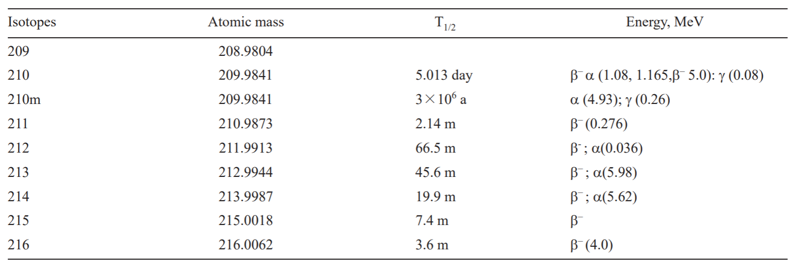
\includegraphics[width=\textwidth]{table-bis-decay-properties} %NAME OF FILE WITHOUT EXTENSION
\end{center}
\end{table}

Lead was also considered because of its excellent neutron properties.  Lead can effectively shield against gamma rays, act as a reflector and absorb few neutrons.  In an accident scenario, lead can potentially still cool the reactor when heated beyond normal operating conditions because of its high boiling point.

\item \textbf{Sodium} 

Sodium has a low ionization energy, which means that it is a high ionization potential.  Due to its high ionization potential, it reacts readily with water to produce sodium hydroxide.  Sodium coolant is reactive with dry hydrogen and water, which would not be ideal for a marine concept.  Even with these flaws, sodium became the preferred choice for fast reactor designs in the 1960s due to a higher power density.  Lead has only one stable isotope, Na-23, and other isotopes of sodium are given in Table 7.  

\begin{table}[H]
\begin{center}
 \caption{Information on the isotopes of sodium and their associated energies emitted upon decay.} \cite{LBE_properties}
 \label{t:lb-decay}  %%SHORT AND MEMORABLE LABEL
 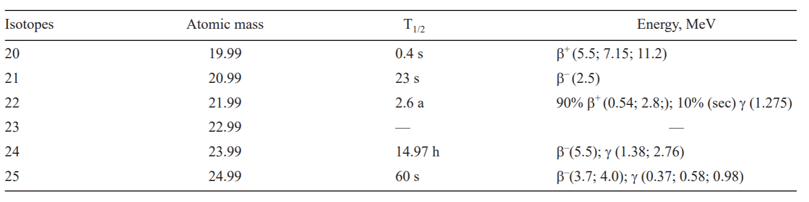
\includegraphics[width=\textwidth]{tab-na-decay-properties} %NAME OF FILE WITHOUT EXTENSION
\end{center}
\end{table}

In Table 7, the isotope Na-23 is responsible for most of the radioactivity in the coolant.  Data for the thermo-physical properties of sodium, lead, bismuth, and lead-bismuth can be seen in Table 8.

\begin{table}[H]
\begin{center}
 \caption{The thermo-physical properties of sodium, lead, bismuth, and lead-bismuth.} \cite{LBE_properties}
 \label{t:lb-decay}  %%SHORT AND MEMORABLE LABEL
 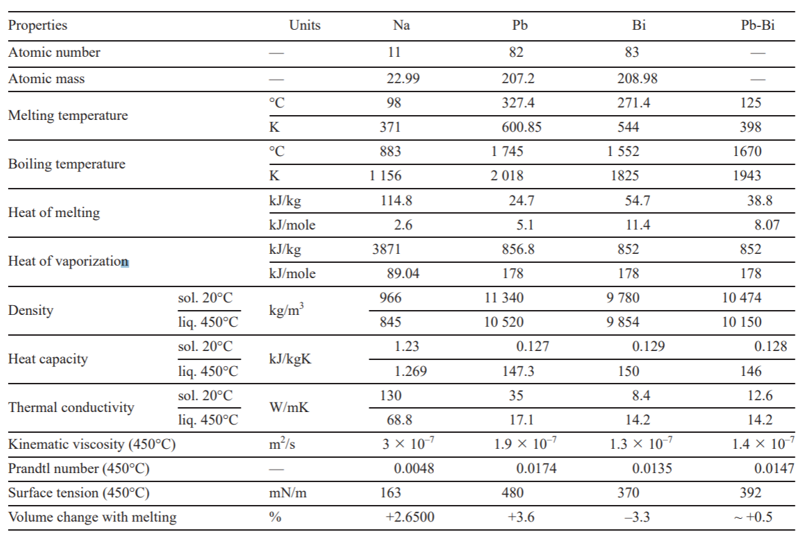
\includegraphics[width=\textwidth]{thermo-props-FR} %NAME OF FILE WITHOUT EXTENSION
\end{center}
\end{table}


  The data in Table 8 indicates there are several benefits and drawbacks of using sodium or lead-bismuth as a fast reactor coolant.  The high thermal conductivity of sodium allows for a higher power density while the lower volume change with melting, viscosity, and resistance to corrosion make lead-bismuth the center of the FISH3P design.

\item \textbf{Water} \newline
	Water was considered as well as a potential coolant for the FISH3P reactor.  This coolant was considered because of the previous research and experimentation with water as a coolant and moderator.  However, the FISH3P reactor utilizes fast neutrons, which makes water a nonoptimal coolant.  The absorption cross section of water and heavy water prevent a breeding reactor’s ability to create a critical neutron environment.  In traditional LWRs, water serves as a moderator and coolant, but moderators slow down fast neutrons.  There is potential for supercritical water to be used as a coolant in fast reactors, but high pressures must be achieved.  
\item \textbf{Gas-Cooled} \newline
	In a gas-cooled reactor, the heat transfer is dictated by the density of the gas.   Helium has been proposed for new reactor designs because of its inert properties, high thermal conductivity for a gas, and low absorption cross section.  Helium can also be used as a coolant for reactors that operate at high temperature outside of the range current LWR technology can manage.  However, helium reactors require special design criteria to reach pressures necessary for operation.
\end{enumerate}
\subsubsection{Fuel}
The FISH3P reactor utilizes different fuel types to achieve its inherently safe design criteria while maintaining criticality.  The materials used in this section of the reactor are discussed below.
\begin{enumerate}
\item \textbf{Inner Core}: \newline
	The inner core of the FISH3P reactor is a cylindrical configuration of UO2 such that the infinite multiplication factor is equal to unity.  The dimensions and enrichment of this fuel are discussed in more detail in the Reactor Concept section.  The inner fuel has been chosen as uranium oxide because it is the largest section of the reactor core.  Choosing this fuel allows for simplicity in materials, neutronics, and economic research because this fuel is currently being used in the current fleet of LWRs.  
	The thermal conductivity of uranium oxide is poor in comparison to uranium metal and other metal fuels.  Poor thermal conductivity in fuel can result in localized overheating in the center of the uranium oxide fuel pellets.  However, utilizing lead-bismuth as a coolant, and the subcritical inner core design will help reduce this effect of power peaking effect.  The thermal conductivity of the inner core will also decrease as a function of temperature.  This temperature effect on the thermal conductivity can be seen in Figure 9.

\begin{figure}[H]                                  
   \centering                                     
    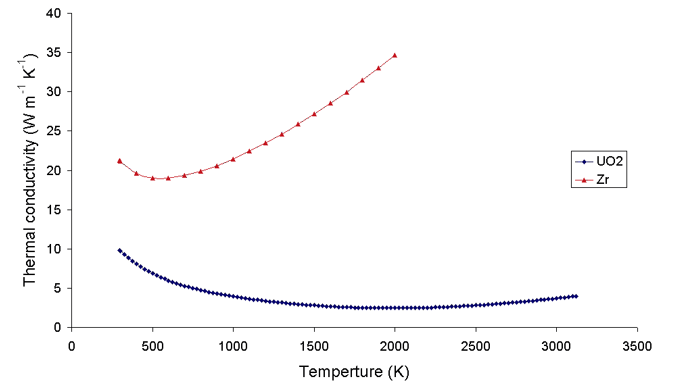
\includegraphics[width=1\textwidth]{themal_cond}   
    \caption{The thermal conductivity of the fuel as a function of temperature} \cite{iaea}        
    \label{fig:mesh1}     
\end{figure}   

\item \textbf{Outer Core}: \newline
Surrounding the subcritical inner core of UO2, the FISH3P design implements a neutron source of fissile material surrounding the inner core.  This material must be liquid so that the reactor maintains its inherently safe design.  To achieve this goal, the neutron source will likely be either a molten salt or pebble fuel design.  The molten salt option has the benefit of becoming a solid at STP, while the pebble-fuel design would allow for online refueling of the outer core.  Once this material is chosen, calculations will be presented in the Reactor Design section.
\item \textbf{Cladding}: \newline
A commonly used form of stainless steel is acid-resistant chrome-nickel steel.  This alloy is referred to as 1Kh18N9T.  The high corrosion resistance and relatively easy welding process because there is no need to heat treat the steel after it welded make it a common choice in marine reactors.  This steel could also possibly be used for pipework, fittings, and water tanks.  Boron can also be added to this particular steel to reduce the yield of capture gamma rays, allowing for the thickness of the shield to decrease.  The steel becomes more brittle with additional boron content, so optimization of boron content and ductility must be considered in the design.

\end{enumerate}

\subsubsection{Shielding}
Shielding materials must be capable of thermalizing neutrons, absorbing the thermal neutrons, and absorb gamma radiation from various energy levels.  There is no one material that has the perfect shielding properties, but some materials are more capable than others for various reactor concepts.  Biological shielding materials have been studied for their potential use in the reactor design.  Various design constraints and overlapping qualities necessitate careful choice to reduce exposure to the crew working on the vessel.  Lead-bismuth and water have been chosen as the current shielding mechanisms in the reactor.  
\begin{enumerate}
\item \textbf{Lead-Bismuth}: \newline
Also serving as a coolant for the reactor, lead-bismuth provides excellent shielding against gamma rays.  However, lead has a dip in the gamma ray absorption cross section at approximately 3 MeV.  This dip in absorption can lead to buildup, which must be taken into consideration in shielding calculations.  Pure lead also does not create neutrons when irradiated.  There are also small amounts of copper, silver, antimony, iron, and zinc in lead.  These materials may create isotopes when irradiated.  If water is used as a secondary shield with the lead, the shielding sections of the reactor may be smaller than other designs provided the lead and steel do not make contact.  
\item \textbf{Water}: \newline
Water can be used as a shield for fast neutrons in this reactor design.  This property can be attributed to the hydrogen content.  However, gamma rays at 2.23 MeV are emitted from the neutron absorption.  This energy range is located where lead has its gamma ray absorption dip, resulting in a thicker lead shield.  Small amounts of boron can be added to the water to reduce the lead shielding thickness. 
\item \textbf{Concrete}: \newline
Concrete can be quite effective as a shielding material because it contains light and heavy nuclei.  The light nuclei provide thermalization of neutrons while the heavy nuclei help with inelastic scattering and absorption of thermal neutrons and gamma rays.  Many additives to concrete have been utilized for different reactor designs so that certain properties are amplified.  For example, iron and lead can be added to concrete to increase its density.  Colemanite can be added to decrease gamma ray yield because it contains boron compounds.  Adequate radiation stability can be achieved by using concrete in the shielding.  
\item \textbf{Polyethylene}: \newline
The high hydrogen content of polyethylene, high softening point, and resistance to acids would 	
make it a candidate for biological shielding, but its low melting temperature, high coefficient of expansion, and ease of ignition disqualify its use.  Its stability is also relatively poor in radioactive conditions, further lowering its melting point.  


\end{enumerate}

\subsubsection{Corrosion}
Material compatibility of lead-bismuth coolant provides a significant challenge to the introduction of these reactors onto the grid.  Russia has experience in developing the LBE coolant technology testing various alloys and maintaining ideal oxygen concentration control to limit corrosion of the steel.  However, there do not seem to be many steels capable of withstanding the lead-bismuth corrosion at high temperatures.  Materials are being developed such as the oxide dispersion steel (ODS) and MAXTHAL which show promise for the reactor type.  However, radiation damage on these materials have not been studied closely so more research needs to be done before it can be determined as the solution.  \newline
The main issue of having lead-bismuth eutectic coolant is the wearing down of the steel surface, moving bits of the piping into the coolant.  The temperature gradient of the coolant loop necessitates the bits of steel to form coatings on the cooler parts of the loop, potentially causing blockages in the coolant flow.  The velocity of the coolant accelerates the corrosion in the piping.  The four types of accelerated corrosion are shown in Figure 10.

\begin{figure}[H]                                  
    \centering                                     
    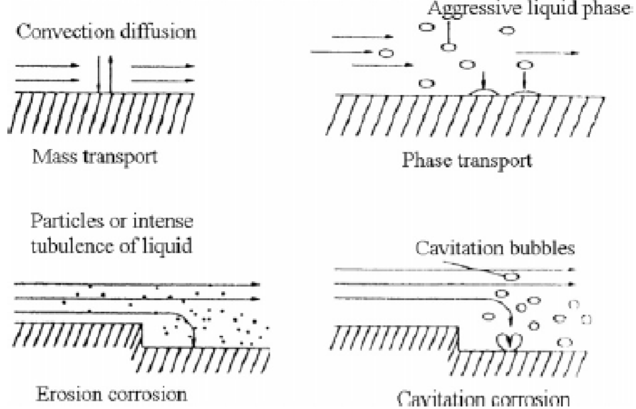
\includegraphics[width=1\textwidth]{corrosion-types}   
    \caption{The four main types of accelerated corrosion the LBE coolant will have on the steel piping.} \cite{Corrosion_LBE}
    \label{fig:mesh1}     
\end{figure}  

If the velocity of the coolant is low, mass transport accelerated corrosion occurs.  Essentially, the dissolution rate of the steel is larger than the mass transfer rate of the steel to the coolant.  When the velocity of the coolant is large, phase transport occurs, which still has the mass transfer of the steel to coolant as dominant corrosion mechanism.  Once the flow becomes very turbulent, the coolant can erode the oxide layer of the steel causing faster corrosion.  This phenomenon is referred to as erosion corrosion.  At even higher velocities, bubbles can form in the coolant and cause cavitation erosion.  This type of corrosion is dangerous because it can quickly corrode small sections of the pipe, endangering the reactor operations.  It would be ideal for the FISH3P to operate with a velocity in the range of the first two listed types of accelerated corrosion.  For this goal to be achieved, more coolant and larger pipes would need to be implemented so that the velocity does not need to increase to turbulent levels.  In doing so, maintenance and reactor lifetime would be extended.


%%%%%%%%%%%%%%%%%%%%%%%%%%%%%%%%%%%%%%%%%%%%%%%%%%%%%%%%%%%%%%%%%%%%%%%%%%%%%%%%


\section{Market analysis}

By designing a marine structure which can act as both a shipping vessel and a power plant, there are many markets in which this project design can enter. Perhaps the most valid option for utilizing this dual-purpose design is through short sea shipping. There are many different areas which utilize short sea shipping throughout the globe. Some of these areas include short sea shipping along the east coast or west coast of the United States, short sea shipping across the great lakes between the United States and Canada, and short sea shipping within the Mediterranean Sea between Europe and Africa. The particular exciting aspect of utilizing FISHP3 for short sea shipping, revolves around the fact that on average, many short sea shipping vessels spend about 50 percent of their time in port. This waiting time could be made more efficient by providing power to the coastal area in which it is residing at the time, alleviating some of the base load power from carbon producing plants. On-peak hour demand levels tend to be highest between 7:00 a.m. and 10:00 p.m. on weekdays, whereas off-peak hour demand levels are generally lowest between 10 p.m. and 7 a.m. and on weekends. If time is utilized properly, FISHP3 could operate as a power provider during on-peak hours and as a shipping vessel during off-peak hours.


However, with this market, there is also some trade off. There are much more carbon emissions produced by ships taking oceanic trade routes over simply coastal ones. This sets back our primary goal of reducing carbon emissions from container vessels at sea. However, this trade off is partially alleviated by the fact that, when the FISHP3 is not participating in carbon-free coastal shipping, it is participating in carbon-free power production. Therefore, we are now cutting into the carbon emissions created from fossil fuel plants on land. Therefore, our overall goal in reducing carbon emissions is still fundamentally intact.


%%%%%%%%%%%%%%%%%%%%%%%%%%%%%%%%%%%%%%%%%%%%%%%%%%%%%%%%%%%%%%%%%%%%%%%%%%%%%%%%
\section{Process planning}
SWOT, Fishikawa, and Gantt charts are provided in this section to give the reader insight into our process planning.
\subsection{SWOT analysis}
\begin{figure}[H]                                  
    \centering                                     
    
\includegraphics[width=1\textwidth]{SWOT}   
   \caption{SWOT analysis for the FISH3P reactor design}                          
   \label{fig:mesh1}     
\end{figure}    
\subsection{Fishikawa}

\begin{figure}[H]                                  
    \centering                                     
    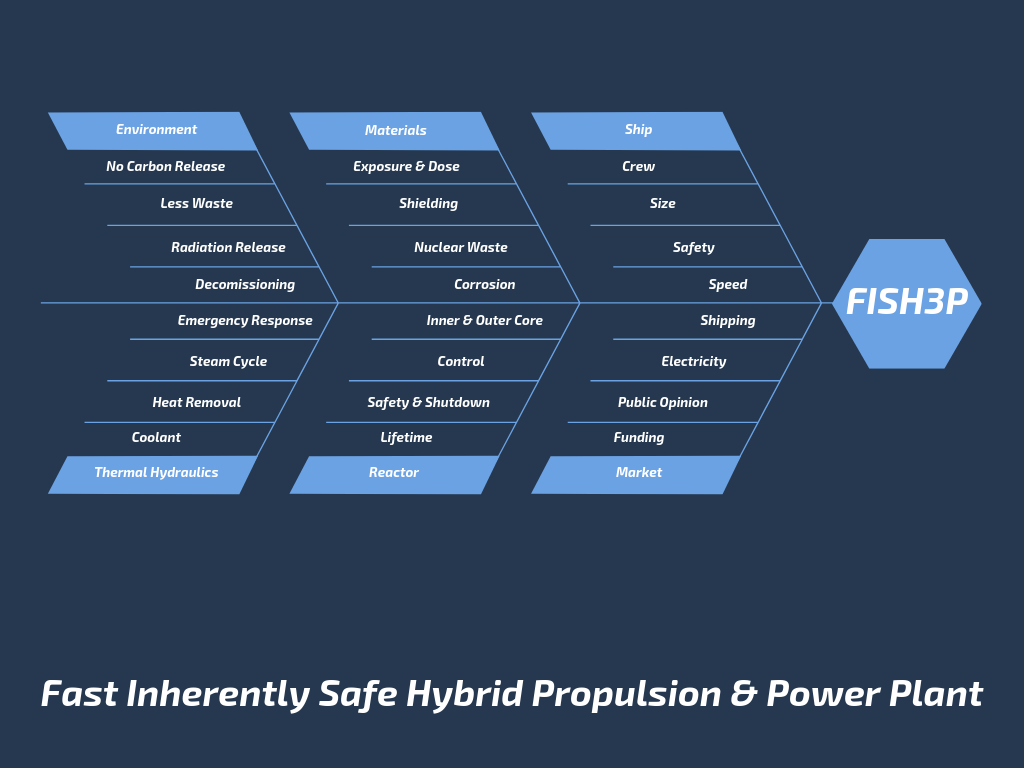
\includegraphics[width=1\textwidth]{fishikawa}   
   \caption{Fishikawa diagram for the FISH3P reactor design}                          
   \label{fig:mesh1}     
\end{figure}                         

\subsection{GANTT chart}
\begin{figure}[H]                                  
    \centering                                     
    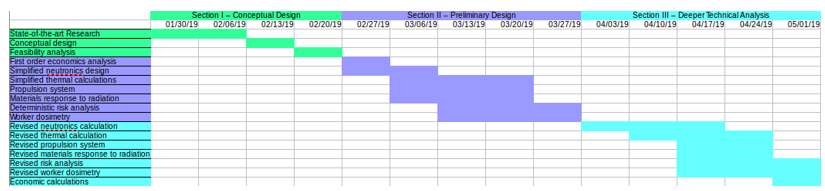
\includegraphics[width=1\textwidth]{gantt-chart}   
   \caption{Gantt chart for the FISH3P reactor design}                          
   \label{fig:mesh1}     
\end{figure}    


%%%%%%%%%%%%%%%%%%%%%%%%%%%%%%%%%%%%%%%%%%%%%%%%%%%%%%%%%%%%%%%%%%%%%%%%%%%%%%%%
\section{Constraints}
We have identified the following set of constraints that will guide the design through the rest of the project:
\begin{itemize}
\item \textbf{Safety}: We seek to meet the definition of ``inherent safety" proposed as a core damage frequency of $10^{-7}$ per year \cite{inherenty_safe}. This goal will be achieved by the driven system as described in previous sections, and will be verified by more detailed analysis in the future. Additionally, the ship itself must meet restrictions on safety defined by the IMO.
\item \textbf{Reliability}: The reactor must be able to scale power enough that Xenon poisoning does not become an issue during navigation at sea.
\item \textbf{Social impact}: To reduce proliferation risk, we hope to fuel the reactor without highly enriched Uranium. Additionally, the system must be manufacturable and operatable without the development of new infrastructures.
\item \textbf{Environmental impact}: We seek to displace harmful gaseous emissions produced by fossil fuels. However, we must ensure throughout our design that the damage caused by potential radioactive release and the manufacturing of the ship, reactor, and fuel does not exceed or approach the damage caused by status quo shipping and electricity generation.
\item \textbf{Sustainability}: The sustainability constraint includes the system's impact on the fuel cycle as well as the cost of its decommissioning. In particular, we seek not to increase the volume of radioactive waste in the United States by more than 10 \% while avoiding a decommissioning disaster such as that experienced in Hunter's Point, California.
\end{itemize}
%%%%%%%%%%%%%%%%%%%%%%%%%%%%%%%%%%%%%%%%%%%%%%%%%%%%%%%%%%%%%%%%%%%%%%%%%%%%%%%%
\section{Conclusions}
The conceptual design has been completed, and feasibility issues regarding the integrity of materials and the viability of LEU fuel in the outer core have been identified. These issues will be addressed by modifying the design concepts and with more detailed calculations. In particular, we hope to propose a core design with a coolant system that is verified by multi-region neutron diffusion calculations in the coming weeks. Additionally, it will be necessary to more rigorously determine the thermal efficiency of our system. The GANTT chart proposed in the ''process planning" section identifies a rough time table for when these calculations will become available. It is also necessary to propose a naval architecture for the ship and to ensure that it meets the safety and social impact constraints identified. 

%%%%%%%%%%%%%%%%%%%%%%%%%%%%%%%%%%%%%%%%%%%%%%%%%%%%%%%%%%%%%%%%%%%%%%%%%%%%%%%%

%%%%%%%%%%%%%%%%%%%%%%%%%%%%%%%%%%%%%%%%%%%%%%%%%%%%%%%%%%%%%%%%%%%%%%%%%%%%%%%%
\section{Acknowledgements}
Thanks to the Illinois NPRE department for their tireless work educating us. In particular, we would like to thank Professor Ragheb for his guidance and mentorship and Professor Stubbins for instructing the Senior Design course.
%%%%%%%%%%%%%%%%%%%%%%%%%%%%%%%%%%%%%%%%%%%%%%%%%%%%%%%%%%%%%%%%%%%%%%%%%%%%%%%%

% \section{Appendices}
% \subsection{Data}
% \subsection{Code}

%%%%%%%%%%%%%%%%%%%%%%%%%%%%%%%%%%%%%%%%%%%%%%%%%%%%%%%%%%%%%%%%%%%%%%%%%%%%%%%%
\section{References}

\bibliographystyle{ans}
\bibliography{bibliography}


%\end{multicols}
\end{document}


%%%%%%%%%%%%%%%%%%%%%%%%%%%%%%%%%%%%		TABLE TEMPLATE
%\begin{table}[H]
%\begin{center}
%  \caption{*} %%DESCRIPTIVE CAPTION
%  \label{t:*}  %%SHORT AND MEMORABLE LABEL
%  \includegraphics[width=0.5\textwidth]{*} %NAME OF FILE WITHOUT EXTENSION
%\end{center}
%\end{table}

%%%%%%%%%%%%%%%%%%%%%%%%%%%%%%%%%%% 		IMAGE TEMPLATE
%\begin{figure}[H]                                  
%    \centering                                     
%    \includegraphics[width=0.25\textwidth]{mesh}   
%    \caption{a nice plot}                          
%    \label{fig:mesh1}     
%\end{figure}                         